\chapter {Network Architecture}
\label{chap:network}

Since the task of image segmentation is a popular one, a number of architecture propositions have been made that aim to produce segmentations. Among them is the \textit{U-Net}, which is the basis of the network used in this thesis.  In the following sections, the Convolutional Neural Network architecture, the differences between this architecture and normal MLPs and the operations in such networks are detailed.


	\section{Convolutional Neural Networks}
\label{sec:CNN}
\textit{Convolutional Neural Networks} (CNNs) are a special subtype of MLPs that were popularized by LeCun \cite{lecun98} and, more recently, the successes of Krizhevsky \cite{krizhevsky2012} in the domain of image classification, although CNNs can be applied to other problems such as sound analysis \cite{CNN_sound} as well, given an adequate mapping of the problem. 

The rationale for their creation was that using fully-connected networks like the ones presented in Section \textbf{\ref{subsec:mlp_backprop}} relate all elements of an input vector to every other element, which is generally a good thing to do. However, this doesn't scale well for very large datasets because of the large number of weights needed. In image data, pixels that are close to each other by some metric are much more likely to be related, while pixels that lie on opposite sides of the image hardly are part of the same pattern, as patterns in images are usually local. Consequently, CNNs encode this spatial relationship by using convolution operations, also called convolutional \textit{layers}, which share weights across all neurons involved in the convolution and thus scale much better.\\

\noindent A \textit{convolution} is a mathematical operation which combines two functions into a new one. Mathematically, a convolution of two functions of a variable $x$ is defined as

\[ f(x) * g(x) = \int \limits_{-\infty}^{\infty} f(u)g(x - u) \, \text{d}u \,, \]

for a dummy variable $u$ that, for instance, denotes time. Convolutions were first used in physical signal processing, but can also be generalized to 2D and 3D spaces, for example to blur images or find contours. In case of an image that is $x \times y$ pixels large, the formula has to be changed to account for the two variables $x$ and $y$ of the image function $I(x, y)$ as well as the fact that pixels are discrete, i.e. not a double integral, but instead a double summation over all pixels is used:

\[ F(x, y) = I(x, y) * g(x, y) = \sum \limits_i \sum \limits_j I(x, y) \, g(x - i, y - j) \,, \] 

In image processing, convolutions on an image are usually performed by defining small, quadratic \textit{kernels} or \textit{weight matrices} with odd dimensions $d \geq 1$, i.e.  $d \times d$ matrices. Using the notation

\[ f(x, y) = g(-x, -y) \,, \]

a values of the kernel matrix are used as the outputs of $f$ and can then be interpreted as the neighborhood weights for some neighborhood of a pixel in $I$. Visualizing the convolution process, the matrix of values of $f$ is aligned with each value in the matrix of values of $I$ by its center value, one after another, and a dot product between the neighborhood from $I$ and the $f$ matrix is calculated, which is then the output of the convolution for the center value. Mathematically, this is expressed by rewriting the convolution formula as

\[ F(x, y) = \sum \limits_i \sum \limits_j I(x + i, y + j) \, f(i, j) \,, \]

which is a more intuitive description of what a convolution amounts to, especially in the context of Figure \textbf{\ref{fig:convolution}}, which shows how a convolution is applied to an image. 

Kernels with even dimensions can also be used. Because there exists no ``real'' center value in the neighborhood, an arbitrary value is chosen instead. For an example of a $2 \times 2$ kernel, one could choose the value to be calculated at each convolution step to be the value corresponding to the top left of the kernel. \cite[pp. 32-33]{machine_vision}\\

However, there also exist definitions of the convolution operation that compute outputs for values in $I$ that are on the border of the matrix, this means that some neighborhood values in $I$ are not defined because the neighborhood would extend over the boundaries of the matrix. In such out-of-bounds cases (OOB), several methods exist to nonetheless perform a convolution. Commonly, OOB values are set to zero and the convolution is performed as usual. An alternative is to treat the matrix like a torus and wrap around once the border is reached.

A normal convolution as defined above thus shrinks the input matrix each time it is applied because it only assigns new values to elements that have a valid neighborhood. For example, if a $3 \times 3$ kernel is used, a 1-value border of the data is lost. This definition of convolution is used in the following sections.\\

\begin {figure}[!htb]
	\begin{center}
		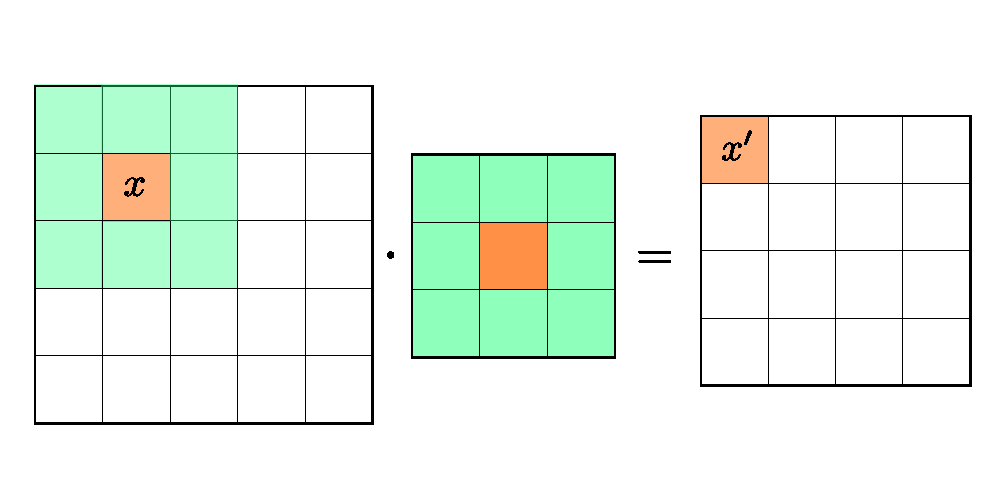
\includegraphics[scale=0.45]{img/fig_convolution}
	\end{center}
	\caption[Matrix convolution.]{A single step of a matrix convolution on an input matrix $I$, using a $3 \times 3$ kernel $f$, producing an output $x'$ in an output matrix $F$. The inspected neighborhood (red, dashed square in $I$ and $f$) of the image value $x$, marked in orange, is given by alignment of $x$ with the kernel center. Note that the output matrix is smaller than the input matrix because values without valid neighborhoods are not calculated.}
	\label{fig:convolution}
\end {figure}

\noindent Concretely, a convolution layer in a CNN typically consists of three sub-components:\footnote{The definition of what a exactly constitutes a ``layer'' is hazy in literature. Sometimes, the subcomponents of a convolutional operation in a neural network are called layers themselves rather than summarizing them. In such cases, ``convolutional layer'' only refers to the part of the operation that actually performs the convolution.}\\

\noindent First, the data is convoluted by applying one or multiple kernels, which are called filters in this context, to all input values and their local neighborhoods. Filters typically have a size of $k \times k \times d$, where $k$ is the filter size and $d$ is the depth of the dataset, e.g. in an RGB image dataset, the depth is 3 because there are 3 color channels. The convolutions performed in CNNs are multi-dimensional in the depth dimension, extending through the whole depth of the stack of input values. The result of these convolutions are as many 2D outputs as there are filters in the layer. These outputs are called \textit{feature maps}, and they then, in turn, provide an input stack for the following layers.

Effectively, applying a specific filter to every valid position in a feature map means that the same pattern is searched in the entire image. Given the right filter weights, a certain pattern creates strong responses and is thus ``recognized'' in the image. Using the same weights for each location in the feature map results in \textit{translation invariance}, i.e. it doesn't matter where the pattern is found for it to be recognized because the response only depends on the weights, not the position of the filter.

After the convolution, the feature maps are passed through a non-linear activation function $h$ to generate ``activation maps'', i.e. a number of activations arranged two-dimensionally. Usually, this combination of convolution and activation is repeated multiple times, using the previous activation maps as input for the next convolution.

\noindent As the third step and last step of a convolutional layer, the generated activation maps are exposed to a pooling operation such as \textit{Maximum Pooling}. Maximum Pooling is a downsampling method that reduces the complexity of the network by replacing groups of values that are apart by a certain stride in the activation map with the maximum value within that group, resulting in a condensed activation map, while performing this calculation for each depth slice of the data independently. Intuitively, some of the information about where a pattern was detected by a filter while creating the feature map is given up in order to make the network easier to manage by reducing the valid convolution filter positions, although the relative spatial relationships between patterns are kept intact. Note that pooling is optional and usually is not performed after each convolution-activation operation, but rather after doing multiple of these (see Section \textbf{\ref{sec:unet}}).

Finally, the resulting downsampled activation maps are fed into a fully-connected layer that calculates a desired number of output values like in a common MLP. \cite[pp. 330-345]{deeplearning_book}\\

\noindent The training of such a network proceeds via Backpropagation as described in Section \textbf{\ref{subsec:mlp_backprop}}, only that the network has to learn the weights of the filters in addition to those of the fully-connected layer. Training the filters results in a hierarchy in which filters that are closer to the input detect low-level features such as edges, while further along the network, filter responses may be triggered by more complex objects only.\\

For an example of a simple CNN architecture, see Figure \textbf{\ref{fig:convnet}}.

\begin {figure}[!htb]
	\begin{flushleft}
		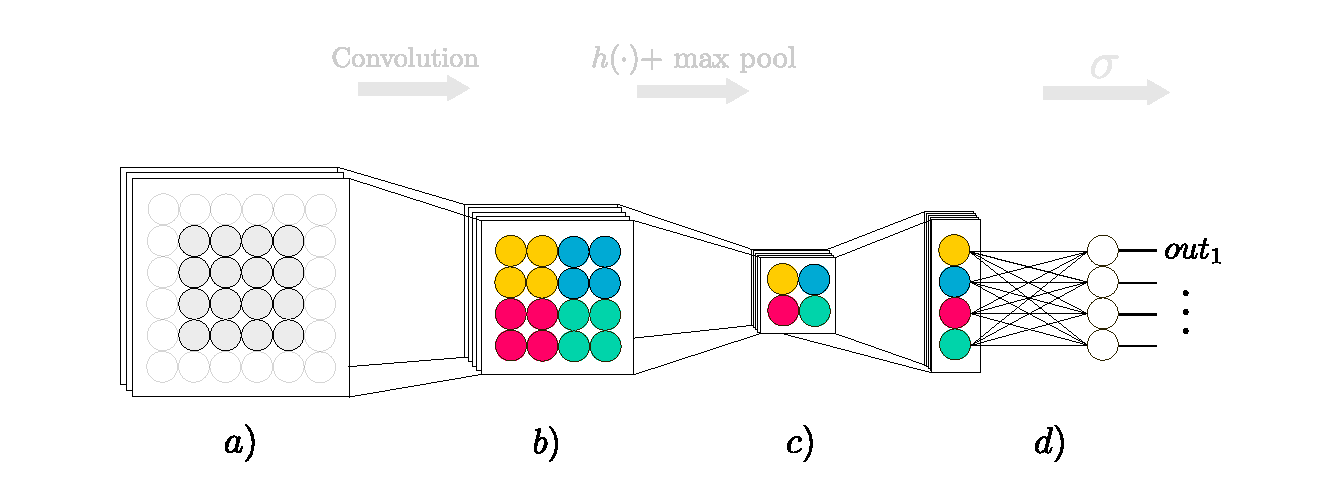
\includegraphics[scale=0.65]{img/fig_convnet}
	\end{flushleft}
	\caption[A small Convolutional Neural Network.]{A small Convolutional Neural Network. For simplicity, most neuron connections are not shown explicitly. \textbf{a):} Input layer. The input size is $6 \times 6 \times 3$, while the filter size is $3 \times 3 \times 3$. Neurons with valid convolution neighborhoods shown in gray. \textbf{b):} Five feature maps with size $4 \times 4 \times 3$ that are the result of applying five different convolution filters to the input, which are then passed into the activation function $h$ to create activation maps. \textbf{c):} Results of a Maximum Pooling operation with sizes $2 \times 2$ and stride $2$ applied to the activation maps. The colors indicate the downsampled position of the maximum activation in a pooling region. \textbf{d):} Fully-connected output layer that calculates the network outputs via applying the output function $\sigma$. The max-pooled values have been rearranged into a column for clarity.}
	\label{fig:convnet}
\end {figure}


	\section {Activation Functions}
Even though previously, the Sigmoid function was given as an example of a suitable activation function for MLPs, recent research \cite{glorot, rectifiers} has shown that better alternatives exist, and it is hardly used anymore. This is mainly because Sigmoids contribute to the problem of ``vanishing gradients'' during Backpropagation, which causes earlier layers in a deep network to train much slower compared to layers near the output layer. ``Vanishing gradients'' happen when the magnitude of the gradient is close to zero, which in turn causes the training to change the network weights in affected layers by only a tiny amount, severely hampering the training progress in these layers.

The Sigmoid function

\[ \sigma(x) = \frac{1}{1 + e^{-x}} \]

\noindent is especially prone to this because its derivative outputs values in the range $\left [0, 1/4 \right ]$ only. Combined with weights initialized to small values, e.g. Gaussian-distributed weights with zero mean and unit variance, the repeated application of the chain rule results in many terms in the range $\left [0, 1\right ]$ being multiplied with each other, leading to very small gradients the closer the algorithm gets to the input layer. The same is true for the $\tanh$ activation function

\begin {align}
	\tanh(x) &= \frac{1 - e^{-2x}}{1 + e^{-2x}}\\
		  &= 2 \left ( \frac{1}{1 + e^{-(2x)}} \right ) - 1\\
		  &= 2 \sigma(2x) - 1
\end {align}

\noindent although its derivative is always in $[0, 1]$ and thus it decays more slowly as it passes through the network. However, in comparison with the Sigmoid, $\tanh$ has the advantage of being zero-centered, because data that is not zero-centered can be detrimental for Gradient Descent training (see Section \textbf{\ref{sec:weight_init}} for more information).\\

In general, activation functions for which

\[ \lim \limits_{x \rightarrow \pm \infty} \frac{\partial}{\partial x} h(x) = 0 \label{eq:saturation} \]

\noindent is true are called \textit{saturating} activation functions and possess the undesirable property of leading to vanishing gradients, which eventually cause problems in the training as the number of network layers increases.\\ 

\noindent A more recent, popular alternative to the Sigmoid and $\tanh$ functions is the \textit{Rectified Linear Unit} function (ReLU). It is defined as the piecewise function

\[  \text{ReLU}(x) = \begin{cases}
			0 \text{ if } x \leq 0\\
			x \text{ else}
		 \end{cases}
\] 

\noindent or simply

\[ \text{ReLU}(x) = \max(0, x) \]

\noindent with its derivative being 

\[ \frac{\partial \text{ReLU}}{\partial x} = \begin{cases}
							1 \text { if } x > 0\\
							0 \text { if } x < 0\\
							 \text{undefined if } x = 0
						        \end{cases} \,,
\]

\noindent although in implementations, the derivative for zero inputs strays from the mathematical definition and is altered to $\frac{\partial \text{ReLU}}{\partial x}\rvert_{x=0} = 0$.\footnote{One example is the ``backward\_cpu'' implementation of the Caffe framework's ReLU layer (\url{https://github.com/BVLC/caffe/blob/master/src/caffe/layers/relu_layer.cpp}).}

ReLUs do not saturate\footnote{This depends on the definition of saturation, for which no standard definition seems to exist. Given the definition in \textbf{\ref{eq:saturation}}, this is true, but since ReLUs cull values below zero, they could also be seen as ``semi-saturating'' functions.} and are cheap to compute compared to activation functions containing exponential expressions, although when using large learning rates and large weights, the gradients can ``explode'' during Backpropagation, which is the opposite of the ``vanishing gradient'' problem. To deal with this, \textit{gradient clipping} can be performed. A popular form of gradient clipping is $L^2$ norm gradient regularization, given by

\[ \hat{g} = \frac{g\,t}{||g||} \,, \]

\noindent where $g$ is the gradient vector, $||g||$ is its $L^2$ norm and $\hat{g}$ is the regularized gradient. This regularization is done whenever $||g||$ is larger than some threshold $t$. \cite{l2clipping}\\

\noindent Despite this, ReLUs still suffer from the problem that they can ``die'' when the network weights are updated in a way that makes them output activation values of zero forever - for example, when a large negative bias term turns all inputs negative and thus results in zero activations. Once a ReLU is dead, the gradient flowing through it will also be zero, and the weights for its neuron won't be updated anymore, which is another form of the saturation problem.

An attempt at fixing this issue is relaxing the strict below-zero activation so it outputs a downscaled version of the input instead. This principle is called \textit{Leaky ReLU} \cite{lrelu} and formally changes the ReLU definition to 

\[  \text{LReLU}(x) = \begin{cases}
			\alpha x \text{ if } x \leq 0\\
			x \text{ else}
		 \end{cases}
\]

\noindent for some small scaling parameter $0 < \alpha < 1$. Consequently, its (zero input-altered) derivative becomes

\[ \frac{\partial \text{LReLU}}{\partial x} = \begin{cases}
							1 \text { if } x > 0\\
							\alpha \text{ else}
						        \end{cases} \,.
\]

\noindent When the leak parameter $\alpha$ is made an additional weight to be trained by Backpropagation, the resulting activation function is called \textit{Parametric ReLU} (PReLU). \cite{rectifiers} Another alternative is the \textit{Exponential ReLU} (ELU), \cite{elu} which aims to combine leakiness with activations close to zero mean to speed up learning. It is defined by

\begin {align}
	\text{ELU}(x) &= \begin{cases}
			x \text { if } x \geq 0\\
			\alpha(e^x - 1) \text{ else}
		     \end{cases}\\
\end {align}

and its derivative 

\begin {align}
	\frac{\partial \text{ELU}}{\partial x} &= \begin{cases}
								1 \text { if } x \geq 0\\
								\text{ELU}(x) + \alpha \text{ else}
		    				     \end{cases} \,,
\end {align}

\noindent where $\alpha$ is a learnable parameter.


\begin {figure}[!htb]
	\begin{center}
	\begin {subfigure}[b]{0.32\linewidth}
		\scalebox{0.65}{%% Creator: Matplotlib, PGF backend
%%
%% To include the figure in your LaTeX document, write
%%   \input{<filename>.pgf}
%%
%% Make sure the required packages are loaded in your preamble
%%   \usepackage{pgf}
%%
%% Figures using additional raster images can only be included by \input if
%% they are in the same directory as the main LaTeX file. For loading figures
%% from other directories you can use the `import` package
%%   \usepackage{import}
%% and then include the figures with
%%   \import{<path to file>}{<filename>.pgf}
%%
%% Matplotlib used the following preamble
%%   \usepackage{fontspec}
%%   \setmainfont{DejaVu Serif}
%%   \setsansfont{DejaVu Sans}
%%   \setmonofont{DejaVu Sans Mono}
%%
\begingroup%
\makeatletter%
\begin{pgfpicture}%
\pgfpathrectangle{\pgfpointorigin}{\pgfqpoint{2.700000in}{2.700000in}}%
\pgfusepath{use as bounding box, clip}%
\begin{pgfscope}%
\pgfsetbuttcap%
\pgfsetmiterjoin%
\definecolor{currentfill}{rgb}{1.000000,1.000000,1.000000}%
\pgfsetfillcolor{currentfill}%
\pgfsetlinewidth{0.000000pt}%
\definecolor{currentstroke}{rgb}{1.000000,1.000000,1.000000}%
\pgfsetstrokecolor{currentstroke}%
\pgfsetdash{}{0pt}%
\pgfpathmoveto{\pgfqpoint{0.000000in}{0.000000in}}%
\pgfpathlineto{\pgfqpoint{2.700000in}{0.000000in}}%
\pgfpathlineto{\pgfqpoint{2.700000in}{2.700000in}}%
\pgfpathlineto{\pgfqpoint{0.000000in}{2.700000in}}%
\pgfpathclose%
\pgfusepath{fill}%
\end{pgfscope}%
\begin{pgfscope}%
\pgfsetbuttcap%
\pgfsetmiterjoin%
\definecolor{currentfill}{rgb}{1.000000,1.000000,1.000000}%
\pgfsetfillcolor{currentfill}%
\pgfsetlinewidth{0.000000pt}%
\definecolor{currentstroke}{rgb}{0.000000,0.000000,0.000000}%
\pgfsetstrokecolor{currentstroke}%
\pgfsetstrokeopacity{0.000000}%
\pgfsetdash{}{0pt}%
\pgfpathmoveto{\pgfqpoint{0.337500in}{0.297000in}}%
\pgfpathlineto{\pgfqpoint{2.430000in}{0.297000in}}%
\pgfpathlineto{\pgfqpoint{2.430000in}{2.376000in}}%
\pgfpathlineto{\pgfqpoint{0.337500in}{2.376000in}}%
\pgfpathclose%
\pgfusepath{fill}%
\end{pgfscope}%
\begin{pgfscope}%
\pgfsetbuttcap%
\pgfsetroundjoin%
\definecolor{currentfill}{rgb}{0.000000,0.000000,0.000000}%
\pgfsetfillcolor{currentfill}%
\pgfsetlinewidth{0.803000pt}%
\definecolor{currentstroke}{rgb}{0.000000,0.000000,0.000000}%
\pgfsetstrokecolor{currentstroke}%
\pgfsetdash{}{0pt}%
\pgfsys@defobject{currentmarker}{\pgfqpoint{0.000000in}{-0.048611in}}{\pgfqpoint{0.000000in}{0.000000in}}{%
\pgfpathmoveto{\pgfqpoint{0.000000in}{0.000000in}}%
\pgfpathlineto{\pgfqpoint{0.000000in}{-0.048611in}}%
\pgfusepath{stroke,fill}%
}%
\begin{pgfscope}%
\pgfsys@transformshift{0.432614in}{0.297000in}%
\pgfsys@useobject{currentmarker}{}%
\end{pgfscope}%
\end{pgfscope}%
\begin{pgfscope}%
\pgftext[x=0.432614in,y=0.199778in,,top]{\sffamily\fontsize{10.000000}{12.000000}\selectfont −5.0}%
\end{pgfscope}%
\begin{pgfscope}%
\pgfsetbuttcap%
\pgfsetroundjoin%
\definecolor{currentfill}{rgb}{0.000000,0.000000,0.000000}%
\pgfsetfillcolor{currentfill}%
\pgfsetlinewidth{0.803000pt}%
\definecolor{currentstroke}{rgb}{0.000000,0.000000,0.000000}%
\pgfsetstrokecolor{currentstroke}%
\pgfsetdash{}{0pt}%
\pgfsys@defobject{currentmarker}{\pgfqpoint{0.000000in}{-0.048611in}}{\pgfqpoint{0.000000in}{0.000000in}}{%
\pgfpathmoveto{\pgfqpoint{0.000000in}{0.000000in}}%
\pgfpathlineto{\pgfqpoint{0.000000in}{-0.048611in}}%
\pgfusepath{stroke,fill}%
}%
\begin{pgfscope}%
\pgfsys@transformshift{0.908658in}{0.297000in}%
\pgfsys@useobject{currentmarker}{}%
\end{pgfscope}%
\end{pgfscope}%
\begin{pgfscope}%
\pgftext[x=0.908658in,y=0.199778in,,top]{\sffamily\fontsize{10.000000}{12.000000}\selectfont −2.5}%
\end{pgfscope}%
\begin{pgfscope}%
\pgfsetbuttcap%
\pgfsetroundjoin%
\definecolor{currentfill}{rgb}{0.000000,0.000000,0.000000}%
\pgfsetfillcolor{currentfill}%
\pgfsetlinewidth{0.803000pt}%
\definecolor{currentstroke}{rgb}{0.000000,0.000000,0.000000}%
\pgfsetstrokecolor{currentstroke}%
\pgfsetdash{}{0pt}%
\pgfsys@defobject{currentmarker}{\pgfqpoint{0.000000in}{-0.048611in}}{\pgfqpoint{0.000000in}{0.000000in}}{%
\pgfpathmoveto{\pgfqpoint{0.000000in}{0.000000in}}%
\pgfpathlineto{\pgfqpoint{0.000000in}{-0.048611in}}%
\pgfusepath{stroke,fill}%
}%
\begin{pgfscope}%
\pgfsys@transformshift{1.384702in}{0.297000in}%
\pgfsys@useobject{currentmarker}{}%
\end{pgfscope}%
\end{pgfscope}%
\begin{pgfscope}%
\pgftext[x=1.384702in,y=0.199778in,,top]{\sffamily\fontsize{10.000000}{12.000000}\selectfont 0.0}%
\end{pgfscope}%
\begin{pgfscope}%
\pgfsetbuttcap%
\pgfsetroundjoin%
\definecolor{currentfill}{rgb}{0.000000,0.000000,0.000000}%
\pgfsetfillcolor{currentfill}%
\pgfsetlinewidth{0.803000pt}%
\definecolor{currentstroke}{rgb}{0.000000,0.000000,0.000000}%
\pgfsetstrokecolor{currentstroke}%
\pgfsetdash{}{0pt}%
\pgfsys@defobject{currentmarker}{\pgfqpoint{0.000000in}{-0.048611in}}{\pgfqpoint{0.000000in}{0.000000in}}{%
\pgfpathmoveto{\pgfqpoint{0.000000in}{0.000000in}}%
\pgfpathlineto{\pgfqpoint{0.000000in}{-0.048611in}}%
\pgfusepath{stroke,fill}%
}%
\begin{pgfscope}%
\pgfsys@transformshift{1.860746in}{0.297000in}%
\pgfsys@useobject{currentmarker}{}%
\end{pgfscope}%
\end{pgfscope}%
\begin{pgfscope}%
\pgftext[x=1.860746in,y=0.199778in,,top]{\sffamily\fontsize{10.000000}{12.000000}\selectfont 2.5}%
\end{pgfscope}%
\begin{pgfscope}%
\pgfsetbuttcap%
\pgfsetroundjoin%
\definecolor{currentfill}{rgb}{0.000000,0.000000,0.000000}%
\pgfsetfillcolor{currentfill}%
\pgfsetlinewidth{0.803000pt}%
\definecolor{currentstroke}{rgb}{0.000000,0.000000,0.000000}%
\pgfsetstrokecolor{currentstroke}%
\pgfsetdash{}{0pt}%
\pgfsys@defobject{currentmarker}{\pgfqpoint{0.000000in}{-0.048611in}}{\pgfqpoint{0.000000in}{0.000000in}}{%
\pgfpathmoveto{\pgfqpoint{0.000000in}{0.000000in}}%
\pgfpathlineto{\pgfqpoint{0.000000in}{-0.048611in}}%
\pgfusepath{stroke,fill}%
}%
\begin{pgfscope}%
\pgfsys@transformshift{2.336791in}{0.297000in}%
\pgfsys@useobject{currentmarker}{}%
\end{pgfscope}%
\end{pgfscope}%
\begin{pgfscope}%
\pgftext[x=2.336791in,y=0.199778in,,top]{\sffamily\fontsize{10.000000}{12.000000}\selectfont 5.0}%
\end{pgfscope}%
\begin{pgfscope}%
\pgfsetbuttcap%
\pgfsetroundjoin%
\definecolor{currentfill}{rgb}{0.000000,0.000000,0.000000}%
\pgfsetfillcolor{currentfill}%
\pgfsetlinewidth{0.803000pt}%
\definecolor{currentstroke}{rgb}{0.000000,0.000000,0.000000}%
\pgfsetstrokecolor{currentstroke}%
\pgfsetdash{}{0pt}%
\pgfsys@defobject{currentmarker}{\pgfqpoint{-0.048611in}{0.000000in}}{\pgfqpoint{0.000000in}{0.000000in}}{%
\pgfpathmoveto{\pgfqpoint{0.000000in}{0.000000in}}%
\pgfpathlineto{\pgfqpoint{-0.048611in}{0.000000in}}%
\pgfusepath{stroke,fill}%
}%
\begin{pgfscope}%
\pgfsys@transformshift{0.337500in}{0.391500in}%
\pgfsys@useobject{currentmarker}{}%
\end{pgfscope}%
\end{pgfscope}%
\begin{pgfscope}%
\pgftext[x=0.019398in,y=0.338738in,left,base]{\sffamily\fontsize{10.000000}{12.000000}\selectfont 0.0}%
\end{pgfscope}%
\begin{pgfscope}%
\pgfsetbuttcap%
\pgfsetroundjoin%
\definecolor{currentfill}{rgb}{0.000000,0.000000,0.000000}%
\pgfsetfillcolor{currentfill}%
\pgfsetlinewidth{0.803000pt}%
\definecolor{currentstroke}{rgb}{0.000000,0.000000,0.000000}%
\pgfsetstrokecolor{currentstroke}%
\pgfsetdash{}{0pt}%
\pgfsys@defobject{currentmarker}{\pgfqpoint{-0.048611in}{0.000000in}}{\pgfqpoint{0.000000in}{0.000000in}}{%
\pgfpathmoveto{\pgfqpoint{0.000000in}{0.000000in}}%
\pgfpathlineto{\pgfqpoint{-0.048611in}{0.000000in}}%
\pgfusepath{stroke,fill}%
}%
\begin{pgfscope}%
\pgfsys@transformshift{0.337500in}{0.772073in}%
\pgfsys@useobject{currentmarker}{}%
\end{pgfscope}%
\end{pgfscope}%
\begin{pgfscope}%
\pgftext[x=0.019398in,y=0.719311in,left,base]{\sffamily\fontsize{10.000000}{12.000000}\selectfont 0.2}%
\end{pgfscope}%
\begin{pgfscope}%
\pgfsetbuttcap%
\pgfsetroundjoin%
\definecolor{currentfill}{rgb}{0.000000,0.000000,0.000000}%
\pgfsetfillcolor{currentfill}%
\pgfsetlinewidth{0.803000pt}%
\definecolor{currentstroke}{rgb}{0.000000,0.000000,0.000000}%
\pgfsetstrokecolor{currentstroke}%
\pgfsetdash{}{0pt}%
\pgfsys@defobject{currentmarker}{\pgfqpoint{-0.048611in}{0.000000in}}{\pgfqpoint{0.000000in}{0.000000in}}{%
\pgfpathmoveto{\pgfqpoint{0.000000in}{0.000000in}}%
\pgfpathlineto{\pgfqpoint{-0.048611in}{0.000000in}}%
\pgfusepath{stroke,fill}%
}%
\begin{pgfscope}%
\pgfsys@transformshift{0.337500in}{1.152645in}%
\pgfsys@useobject{currentmarker}{}%
\end{pgfscope}%
\end{pgfscope}%
\begin{pgfscope}%
\pgftext[x=0.019398in,y=1.099884in,left,base]{\sffamily\fontsize{10.000000}{12.000000}\selectfont 0.4}%
\end{pgfscope}%
\begin{pgfscope}%
\pgfsetbuttcap%
\pgfsetroundjoin%
\definecolor{currentfill}{rgb}{0.000000,0.000000,0.000000}%
\pgfsetfillcolor{currentfill}%
\pgfsetlinewidth{0.803000pt}%
\definecolor{currentstroke}{rgb}{0.000000,0.000000,0.000000}%
\pgfsetstrokecolor{currentstroke}%
\pgfsetdash{}{0pt}%
\pgfsys@defobject{currentmarker}{\pgfqpoint{-0.048611in}{0.000000in}}{\pgfqpoint{0.000000in}{0.000000in}}{%
\pgfpathmoveto{\pgfqpoint{0.000000in}{0.000000in}}%
\pgfpathlineto{\pgfqpoint{-0.048611in}{0.000000in}}%
\pgfusepath{stroke,fill}%
}%
\begin{pgfscope}%
\pgfsys@transformshift{0.337500in}{1.533218in}%
\pgfsys@useobject{currentmarker}{}%
\end{pgfscope}%
\end{pgfscope}%
\begin{pgfscope}%
\pgftext[x=0.019398in,y=1.480456in,left,base]{\sffamily\fontsize{10.000000}{12.000000}\selectfont 0.6}%
\end{pgfscope}%
\begin{pgfscope}%
\pgfsetbuttcap%
\pgfsetroundjoin%
\definecolor{currentfill}{rgb}{0.000000,0.000000,0.000000}%
\pgfsetfillcolor{currentfill}%
\pgfsetlinewidth{0.803000pt}%
\definecolor{currentstroke}{rgb}{0.000000,0.000000,0.000000}%
\pgfsetstrokecolor{currentstroke}%
\pgfsetdash{}{0pt}%
\pgfsys@defobject{currentmarker}{\pgfqpoint{-0.048611in}{0.000000in}}{\pgfqpoint{0.000000in}{0.000000in}}{%
\pgfpathmoveto{\pgfqpoint{0.000000in}{0.000000in}}%
\pgfpathlineto{\pgfqpoint{-0.048611in}{0.000000in}}%
\pgfusepath{stroke,fill}%
}%
\begin{pgfscope}%
\pgfsys@transformshift{0.337500in}{1.913790in}%
\pgfsys@useobject{currentmarker}{}%
\end{pgfscope}%
\end{pgfscope}%
\begin{pgfscope}%
\pgftext[x=0.019398in,y=1.861029in,left,base]{\sffamily\fontsize{10.000000}{12.000000}\selectfont 0.8}%
\end{pgfscope}%
\begin{pgfscope}%
\pgfsetbuttcap%
\pgfsetroundjoin%
\definecolor{currentfill}{rgb}{0.000000,0.000000,0.000000}%
\pgfsetfillcolor{currentfill}%
\pgfsetlinewidth{0.803000pt}%
\definecolor{currentstroke}{rgb}{0.000000,0.000000,0.000000}%
\pgfsetstrokecolor{currentstroke}%
\pgfsetdash{}{0pt}%
\pgfsys@defobject{currentmarker}{\pgfqpoint{-0.048611in}{0.000000in}}{\pgfqpoint{0.000000in}{0.000000in}}{%
\pgfpathmoveto{\pgfqpoint{0.000000in}{0.000000in}}%
\pgfpathlineto{\pgfqpoint{-0.048611in}{0.000000in}}%
\pgfusepath{stroke,fill}%
}%
\begin{pgfscope}%
\pgfsys@transformshift{0.337500in}{2.294363in}%
\pgfsys@useobject{currentmarker}{}%
\end{pgfscope}%
\end{pgfscope}%
\begin{pgfscope}%
\pgftext[x=0.019398in,y=2.241601in,left,base]{\sffamily\fontsize{10.000000}{12.000000}\selectfont 1.0}%
\end{pgfscope}%
\begin{pgfscope}%
\pgfpathrectangle{\pgfqpoint{0.337500in}{0.297000in}}{\pgfqpoint{2.092500in}{2.079000in}} %
\pgfusepath{clip}%
\pgfsetrectcap%
\pgfsetroundjoin%
\pgfsetlinewidth{1.505625pt}%
\definecolor{currentstroke}{rgb}{0.000000,0.000000,0.000000}%
\pgfsetstrokecolor{currentstroke}%
\pgfsetstrokeopacity{0.250000}%
\pgfsetdash{}{0pt}%
\pgfpathmoveto{\pgfqpoint{0.337500in}{0.391500in}}%
\pgfpathlineto{\pgfqpoint{2.430000in}{0.391500in}}%
\pgfusepath{stroke}%
\end{pgfscope}%
\begin{pgfscope}%
\pgfpathrectangle{\pgfqpoint{0.337500in}{0.297000in}}{\pgfqpoint{2.092500in}{2.079000in}} %
\pgfusepath{clip}%
\pgfsetrectcap%
\pgfsetroundjoin%
\pgfsetlinewidth{1.505625pt}%
\definecolor{currentstroke}{rgb}{0.000000,0.000000,0.000000}%
\pgfsetstrokecolor{currentstroke}%
\pgfsetstrokeopacity{0.250000}%
\pgfsetdash{}{0pt}%
\pgfpathmoveto{\pgfqpoint{1.384702in}{0.297000in}}%
\pgfpathlineto{\pgfqpoint{1.384702in}{2.376000in}}%
\pgfusepath{stroke}%
\end{pgfscope}%
\begin{pgfscope}%
\pgfpathrectangle{\pgfqpoint{0.337500in}{0.297000in}}{\pgfqpoint{2.092500in}{2.079000in}} %
\pgfusepath{clip}%
\pgfsetrectcap%
\pgfsetroundjoin%
\pgfsetlinewidth{1.505625pt}%
\definecolor{currentstroke}{rgb}{0.274510,0.509804,0.705882}%
\pgfsetstrokecolor{currentstroke}%
\pgfsetdash{}{0pt}%
\pgfpathmoveto{\pgfqpoint{0.432614in}{0.404236in}}%
\pgfpathlineto{\pgfqpoint{0.506877in}{0.410250in}}%
\pgfpathlineto{\pgfqpoint{0.569714in}{0.417481in}}%
\pgfpathlineto{\pgfqpoint{0.624936in}{0.426063in}}%
\pgfpathlineto{\pgfqpoint{0.672540in}{0.435652in}}%
\pgfpathlineto{\pgfqpoint{0.716336in}{0.446738in}}%
\pgfpathlineto{\pgfqpoint{0.756324in}{0.459187in}}%
\pgfpathlineto{\pgfqpoint{0.792503in}{0.472746in}}%
\pgfpathlineto{\pgfqpoint{0.826778in}{0.487957in}}%
\pgfpathlineto{\pgfqpoint{0.859149in}{0.504767in}}%
\pgfpathlineto{\pgfqpoint{0.889616in}{0.523061in}}%
\pgfpathlineto{\pgfqpoint{0.920083in}{0.544058in}}%
\pgfpathlineto{\pgfqpoint{0.948646in}{0.566477in}}%
\pgfpathlineto{\pgfqpoint{0.977208in}{0.591813in}}%
\pgfpathlineto{\pgfqpoint{1.003867in}{0.618327in}}%
\pgfpathlineto{\pgfqpoint{1.030525in}{0.647821in}}%
\pgfpathlineto{\pgfqpoint{1.057184in}{0.680490in}}%
\pgfpathlineto{\pgfqpoint{1.083842in}{0.716500in}}%
\pgfpathlineto{\pgfqpoint{1.112405in}{0.758940in}}%
\pgfpathlineto{\pgfqpoint{1.140967in}{0.805468in}}%
\pgfpathlineto{\pgfqpoint{1.171434in}{0.859626in}}%
\pgfpathlineto{\pgfqpoint{1.201901in}{0.918361in}}%
\pgfpathlineto{\pgfqpoint{1.234272in}{0.985514in}}%
\pgfpathlineto{\pgfqpoint{1.270451in}{1.065767in}}%
\pgfpathlineto{\pgfqpoint{1.312343in}{1.164304in}}%
\pgfpathlineto{\pgfqpoint{1.369469in}{1.304894in}}%
\pgfpathlineto{\pgfqpoint{1.468486in}{1.548933in}}%
\pgfpathlineto{\pgfqpoint{1.512282in}{1.650250in}}%
\pgfpathlineto{\pgfqpoint{1.548461in}{1.728567in}}%
\pgfpathlineto{\pgfqpoint{1.582736in}{1.797430in}}%
\pgfpathlineto{\pgfqpoint{1.613203in}{1.853897in}}%
\pgfpathlineto{\pgfqpoint{1.643670in}{1.905721in}}%
\pgfpathlineto{\pgfqpoint{1.672233in}{1.950061in}}%
\pgfpathlineto{\pgfqpoint{1.700795in}{1.990358in}}%
\pgfpathlineto{\pgfqpoint{1.729358in}{2.026748in}}%
\pgfpathlineto{\pgfqpoint{1.757921in}{2.059422in}}%
\pgfpathlineto{\pgfqpoint{1.786483in}{2.088609in}}%
\pgfpathlineto{\pgfqpoint{1.815046in}{2.114561in}}%
\pgfpathlineto{\pgfqpoint{1.843609in}{2.137541in}}%
\pgfpathlineto{\pgfqpoint{1.874076in}{2.159080in}}%
\pgfpathlineto{\pgfqpoint{1.904542in}{2.177858in}}%
\pgfpathlineto{\pgfqpoint{1.936913in}{2.195122in}}%
\pgfpathlineto{\pgfqpoint{1.971189in}{2.210751in}}%
\pgfpathlineto{\pgfqpoint{2.007368in}{2.224690in}}%
\pgfpathlineto{\pgfqpoint{2.045451in}{2.236938in}}%
\pgfpathlineto{\pgfqpoint{2.087343in}{2.248002in}}%
\pgfpathlineto{\pgfqpoint{2.133044in}{2.257704in}}%
\pgfpathlineto{\pgfqpoint{2.184456in}{2.266250in}}%
\pgfpathlineto{\pgfqpoint{2.241582in}{2.273456in}}%
\pgfpathlineto{\pgfqpoint{2.308228in}{2.279582in}}%
\pgfpathlineto{\pgfqpoint{2.334886in}{2.281500in}}%
\pgfpathlineto{\pgfqpoint{2.334886in}{2.281500in}}%
\pgfusepath{stroke}%
\end{pgfscope}%
\begin{pgfscope}%
\pgfpathrectangle{\pgfqpoint{0.337500in}{0.297000in}}{\pgfqpoint{2.092500in}{2.079000in}} %
\pgfusepath{clip}%
\pgfsetrectcap%
\pgfsetroundjoin%
\pgfsetlinewidth{1.505625pt}%
\definecolor{currentstroke}{rgb}{1.000000,0.647059,0.000000}%
\pgfsetstrokecolor{currentstroke}%
\pgfsetdash{}{0pt}%
\pgfpathmoveto{\pgfqpoint{0.432614in}{0.404150in}}%
\pgfpathlineto{\pgfqpoint{0.508781in}{0.410248in}}%
\pgfpathlineto{\pgfqpoint{0.573523in}{0.417630in}}%
\pgfpathlineto{\pgfqpoint{0.628744in}{0.426095in}}%
\pgfpathlineto{\pgfqpoint{0.678252in}{0.435878in}}%
\pgfpathlineto{\pgfqpoint{0.723953in}{0.447192in}}%
\pgfpathlineto{\pgfqpoint{0.765845in}{0.459877in}}%
\pgfpathlineto{\pgfqpoint{0.803928in}{0.473652in}}%
\pgfpathlineto{\pgfqpoint{0.840107in}{0.488989in}}%
\pgfpathlineto{\pgfqpoint{0.876287in}{0.506761in}}%
\pgfpathlineto{\pgfqpoint{0.910562in}{0.526033in}}%
\pgfpathlineto{\pgfqpoint{0.944837in}{0.547809in}}%
\pgfpathlineto{\pgfqpoint{0.979112in}{0.572145in}}%
\pgfpathlineto{\pgfqpoint{1.015292in}{0.600549in}}%
\pgfpathlineto{\pgfqpoint{1.055279in}{0.634897in}}%
\pgfpathlineto{\pgfqpoint{1.102884in}{0.678916in}}%
\pgfpathlineto{\pgfqpoint{1.215230in}{0.784184in}}%
\pgfpathlineto{\pgfqpoint{1.245697in}{0.809070in}}%
\pgfpathlineto{\pgfqpoint{1.272356in}{0.828105in}}%
\pgfpathlineto{\pgfqpoint{1.295206in}{0.841882in}}%
\pgfpathlineto{\pgfqpoint{1.316152in}{0.852129in}}%
\pgfpathlineto{\pgfqpoint{1.337098in}{0.859859in}}%
\pgfpathlineto{\pgfqpoint{1.356139in}{0.864550in}}%
\pgfpathlineto{\pgfqpoint{1.375181in}{0.866918in}}%
\pgfpathlineto{\pgfqpoint{1.394223in}{0.866918in}}%
\pgfpathlineto{\pgfqpoint{1.413265in}{0.864550in}}%
\pgfpathlineto{\pgfqpoint{1.432307in}{0.859859in}}%
\pgfpathlineto{\pgfqpoint{1.451348in}{0.852939in}}%
\pgfpathlineto{\pgfqpoint{1.472294in}{0.842912in}}%
\pgfpathlineto{\pgfqpoint{1.495144in}{0.829349in}}%
\pgfpathlineto{\pgfqpoint{1.519899in}{0.811963in}}%
\pgfpathlineto{\pgfqpoint{1.548461in}{0.789063in}}%
\pgfpathlineto{\pgfqpoint{1.584641in}{0.756902in}}%
\pgfpathlineto{\pgfqpoint{1.643670in}{0.700765in}}%
\pgfpathlineto{\pgfqpoint{1.708412in}{0.640025in}}%
\pgfpathlineto{\pgfqpoint{1.750304in}{0.603694in}}%
\pgfpathlineto{\pgfqpoint{1.788388in}{0.573572in}}%
\pgfpathlineto{\pgfqpoint{1.824567in}{0.547809in}}%
\pgfpathlineto{\pgfqpoint{1.858842in}{0.526033in}}%
\pgfpathlineto{\pgfqpoint{1.893117in}{0.506761in}}%
\pgfpathlineto{\pgfqpoint{1.929297in}{0.488989in}}%
\pgfpathlineto{\pgfqpoint{1.965476in}{0.473652in}}%
\pgfpathlineto{\pgfqpoint{2.003560in}{0.459877in}}%
\pgfpathlineto{\pgfqpoint{2.043547in}{0.447717in}}%
\pgfpathlineto{\pgfqpoint{2.087343in}{0.436731in}}%
\pgfpathlineto{\pgfqpoint{2.134948in}{0.427109in}}%
\pgfpathlineto{\pgfqpoint{2.188265in}{0.418665in}}%
\pgfpathlineto{\pgfqpoint{2.249198in}{0.411383in}}%
\pgfpathlineto{\pgfqpoint{2.319653in}{0.405324in}}%
\pgfpathlineto{\pgfqpoint{2.334886in}{0.404276in}}%
\pgfpathlineto{\pgfqpoint{2.334886in}{0.404276in}}%
\pgfusepath{stroke}%
\end{pgfscope}%
\begin{pgfscope}%
\pgfsetrectcap%
\pgfsetmiterjoin%
\pgfsetlinewidth{0.803000pt}%
\definecolor{currentstroke}{rgb}{0.000000,0.000000,0.000000}%
\pgfsetstrokecolor{currentstroke}%
\pgfsetdash{}{0pt}%
\pgfpathmoveto{\pgfqpoint{0.337500in}{0.297000in}}%
\pgfpathlineto{\pgfqpoint{0.337500in}{2.376000in}}%
\pgfusepath{stroke}%
\end{pgfscope}%
\begin{pgfscope}%
\pgfsetrectcap%
\pgfsetmiterjoin%
\pgfsetlinewidth{0.803000pt}%
\definecolor{currentstroke}{rgb}{0.000000,0.000000,0.000000}%
\pgfsetstrokecolor{currentstroke}%
\pgfsetdash{}{0pt}%
\pgfpathmoveto{\pgfqpoint{2.430000in}{0.297000in}}%
\pgfpathlineto{\pgfqpoint{2.430000in}{2.376000in}}%
\pgfusepath{stroke}%
\end{pgfscope}%
\begin{pgfscope}%
\pgfsetrectcap%
\pgfsetmiterjoin%
\pgfsetlinewidth{0.803000pt}%
\definecolor{currentstroke}{rgb}{0.000000,0.000000,0.000000}%
\pgfsetstrokecolor{currentstroke}%
\pgfsetdash{}{0pt}%
\pgfpathmoveto{\pgfqpoint{0.337500in}{0.297000in}}%
\pgfpathlineto{\pgfqpoint{2.430000in}{0.297000in}}%
\pgfusepath{stroke}%
\end{pgfscope}%
\begin{pgfscope}%
\pgfsetrectcap%
\pgfsetmiterjoin%
\pgfsetlinewidth{0.803000pt}%
\definecolor{currentstroke}{rgb}{0.000000,0.000000,0.000000}%
\pgfsetstrokecolor{currentstroke}%
\pgfsetdash{}{0pt}%
\pgfpathmoveto{\pgfqpoint{0.337500in}{2.376000in}}%
\pgfpathlineto{\pgfqpoint{2.430000in}{2.376000in}}%
\pgfusepath{stroke}%
\end{pgfscope}%
\end{pgfpicture}%
\makeatother%
\endgroup%
}
		\caption{}
	\end {subfigure}
	\begin {subfigure}[b]{0.32\linewidth}
		\scalebox{0.65}{%% Creator: Matplotlib, PGF backend
%%
%% To include the figure in your LaTeX document, write
%%   \input{<filename>.pgf}
%%
%% Make sure the required packages are loaded in your preamble
%%   \usepackage{pgf}
%%
%% Figures using additional raster images can only be included by \input if
%% they are in the same directory as the main LaTeX file. For loading figures
%% from other directories you can use the `import` package
%%   \usepackage{import}
%% and then include the figures with
%%   \import{<path to file>}{<filename>.pgf}
%%
%% Matplotlib used the following preamble
%%   \usepackage{fontspec}
%%   \setmainfont{DejaVu Serif}
%%   \setsansfont{DejaVu Sans}
%%   \setmonofont{DejaVu Sans Mono}
%%
\begingroup%
\makeatletter%
\begin{pgfpicture}%
\pgfpathrectangle{\pgfpointorigin}{\pgfqpoint{2.700000in}{2.700000in}}%
\pgfusepath{use as bounding box, clip}%
\begin{pgfscope}%
\pgfsetbuttcap%
\pgfsetmiterjoin%
\definecolor{currentfill}{rgb}{1.000000,1.000000,1.000000}%
\pgfsetfillcolor{currentfill}%
\pgfsetlinewidth{0.000000pt}%
\definecolor{currentstroke}{rgb}{1.000000,1.000000,1.000000}%
\pgfsetstrokecolor{currentstroke}%
\pgfsetdash{}{0pt}%
\pgfpathmoveto{\pgfqpoint{0.000000in}{0.000000in}}%
\pgfpathlineto{\pgfqpoint{2.700000in}{0.000000in}}%
\pgfpathlineto{\pgfqpoint{2.700000in}{2.700000in}}%
\pgfpathlineto{\pgfqpoint{0.000000in}{2.700000in}}%
\pgfpathclose%
\pgfusepath{fill}%
\end{pgfscope}%
\begin{pgfscope}%
\pgfsetbuttcap%
\pgfsetmiterjoin%
\definecolor{currentfill}{rgb}{1.000000,1.000000,1.000000}%
\pgfsetfillcolor{currentfill}%
\pgfsetlinewidth{0.000000pt}%
\definecolor{currentstroke}{rgb}{0.000000,0.000000,0.000000}%
\pgfsetstrokecolor{currentstroke}%
\pgfsetstrokeopacity{0.000000}%
\pgfsetdash{}{0pt}%
\pgfpathmoveto{\pgfqpoint{0.780278in}{0.582778in}}%
\pgfpathlineto{\pgfqpoint{2.515000in}{0.582778in}}%
\pgfpathlineto{\pgfqpoint{2.515000in}{2.515000in}}%
\pgfpathlineto{\pgfqpoint{0.780278in}{2.515000in}}%
\pgfpathclose%
\pgfusepath{fill}%
\end{pgfscope}%
\begin{pgfscope}%
\pgfsetbuttcap%
\pgfsetroundjoin%
\definecolor{currentfill}{rgb}{0.000000,0.000000,0.000000}%
\pgfsetfillcolor{currentfill}%
\pgfsetlinewidth{0.803000pt}%
\definecolor{currentstroke}{rgb}{0.000000,0.000000,0.000000}%
\pgfsetstrokecolor{currentstroke}%
\pgfsetdash{}{0pt}%
\pgfsys@defobject{currentmarker}{\pgfqpoint{0.000000in}{-0.048611in}}{\pgfqpoint{0.000000in}{0.000000in}}{%
\pgfpathmoveto{\pgfqpoint{0.000000in}{0.000000in}}%
\pgfpathlineto{\pgfqpoint{0.000000in}{-0.048611in}}%
\pgfusepath{stroke,fill}%
}%
\begin{pgfscope}%
\pgfsys@transformshift{0.859129in}{0.582778in}%
\pgfsys@useobject{currentmarker}{}%
\end{pgfscope}%
\end{pgfscope}%
\begin{pgfscope}%
\pgftext[x=0.859129in,y=0.485556in,,top]{\sffamily\fontsize{10.000000}{12.000000}\selectfont −5.0}%
\end{pgfscope}%
\begin{pgfscope}%
\pgfsetbuttcap%
\pgfsetroundjoin%
\definecolor{currentfill}{rgb}{0.000000,0.000000,0.000000}%
\pgfsetfillcolor{currentfill}%
\pgfsetlinewidth{0.803000pt}%
\definecolor{currentstroke}{rgb}{0.000000,0.000000,0.000000}%
\pgfsetstrokecolor{currentstroke}%
\pgfsetdash{}{0pt}%
\pgfsys@defobject{currentmarker}{\pgfqpoint{0.000000in}{-0.048611in}}{\pgfqpoint{0.000000in}{0.000000in}}{%
\pgfpathmoveto{\pgfqpoint{0.000000in}{0.000000in}}%
\pgfpathlineto{\pgfqpoint{0.000000in}{-0.048611in}}%
\pgfusepath{stroke,fill}%
}%
\begin{pgfscope}%
\pgfsys@transformshift{1.253778in}{0.582778in}%
\pgfsys@useobject{currentmarker}{}%
\end{pgfscope}%
\end{pgfscope}%
\begin{pgfscope}%
\pgftext[x=1.253778in,y=0.485556in,,top]{\sffamily\fontsize{10.000000}{12.000000}\selectfont −2.5}%
\end{pgfscope}%
\begin{pgfscope}%
\pgfsetbuttcap%
\pgfsetroundjoin%
\definecolor{currentfill}{rgb}{0.000000,0.000000,0.000000}%
\pgfsetfillcolor{currentfill}%
\pgfsetlinewidth{0.803000pt}%
\definecolor{currentstroke}{rgb}{0.000000,0.000000,0.000000}%
\pgfsetstrokecolor{currentstroke}%
\pgfsetdash{}{0pt}%
\pgfsys@defobject{currentmarker}{\pgfqpoint{0.000000in}{-0.048611in}}{\pgfqpoint{0.000000in}{0.000000in}}{%
\pgfpathmoveto{\pgfqpoint{0.000000in}{0.000000in}}%
\pgfpathlineto{\pgfqpoint{0.000000in}{-0.048611in}}%
\pgfusepath{stroke,fill}%
}%
\begin{pgfscope}%
\pgfsys@transformshift{1.648428in}{0.582778in}%
\pgfsys@useobject{currentmarker}{}%
\end{pgfscope}%
\end{pgfscope}%
\begin{pgfscope}%
\pgftext[x=1.648428in,y=0.485556in,,top]{\sffamily\fontsize{10.000000}{12.000000}\selectfont 0.0}%
\end{pgfscope}%
\begin{pgfscope}%
\pgfsetbuttcap%
\pgfsetroundjoin%
\definecolor{currentfill}{rgb}{0.000000,0.000000,0.000000}%
\pgfsetfillcolor{currentfill}%
\pgfsetlinewidth{0.803000pt}%
\definecolor{currentstroke}{rgb}{0.000000,0.000000,0.000000}%
\pgfsetstrokecolor{currentstroke}%
\pgfsetdash{}{0pt}%
\pgfsys@defobject{currentmarker}{\pgfqpoint{0.000000in}{-0.048611in}}{\pgfqpoint{0.000000in}{0.000000in}}{%
\pgfpathmoveto{\pgfqpoint{0.000000in}{0.000000in}}%
\pgfpathlineto{\pgfqpoint{0.000000in}{-0.048611in}}%
\pgfusepath{stroke,fill}%
}%
\begin{pgfscope}%
\pgfsys@transformshift{2.043078in}{0.582778in}%
\pgfsys@useobject{currentmarker}{}%
\end{pgfscope}%
\end{pgfscope}%
\begin{pgfscope}%
\pgftext[x=2.043078in,y=0.485556in,,top]{\sffamily\fontsize{10.000000}{12.000000}\selectfont 2.5}%
\end{pgfscope}%
\begin{pgfscope}%
\pgfsetbuttcap%
\pgfsetroundjoin%
\definecolor{currentfill}{rgb}{0.000000,0.000000,0.000000}%
\pgfsetfillcolor{currentfill}%
\pgfsetlinewidth{0.803000pt}%
\definecolor{currentstroke}{rgb}{0.000000,0.000000,0.000000}%
\pgfsetstrokecolor{currentstroke}%
\pgfsetdash{}{0pt}%
\pgfsys@defobject{currentmarker}{\pgfqpoint{0.000000in}{-0.048611in}}{\pgfqpoint{0.000000in}{0.000000in}}{%
\pgfpathmoveto{\pgfqpoint{0.000000in}{0.000000in}}%
\pgfpathlineto{\pgfqpoint{0.000000in}{-0.048611in}}%
\pgfusepath{stroke,fill}%
}%
\begin{pgfscope}%
\pgfsys@transformshift{2.437728in}{0.582778in}%
\pgfsys@useobject{currentmarker}{}%
\end{pgfscope}%
\end{pgfscope}%
\begin{pgfscope}%
\pgftext[x=2.437728in,y=0.485556in,,top]{\sffamily\fontsize{10.000000}{12.000000}\selectfont 5.0}%
\end{pgfscope}%
\begin{pgfscope}%
\pgftext[x=1.647639in,y=0.295587in,,top]{\sffamily\fontsize{10.000000}{12.000000}\selectfont x}%
\end{pgfscope}%
\begin{pgfscope}%
\pgfsetbuttcap%
\pgfsetroundjoin%
\definecolor{currentfill}{rgb}{0.000000,0.000000,0.000000}%
\pgfsetfillcolor{currentfill}%
\pgfsetlinewidth{0.803000pt}%
\definecolor{currentstroke}{rgb}{0.000000,0.000000,0.000000}%
\pgfsetstrokecolor{currentstroke}%
\pgfsetdash{}{0pt}%
\pgfsys@defobject{currentmarker}{\pgfqpoint{-0.048611in}{0.000000in}}{\pgfqpoint{0.000000in}{0.000000in}}{%
\pgfpathmoveto{\pgfqpoint{0.000000in}{0.000000in}}%
\pgfpathlineto{\pgfqpoint{-0.048611in}{0.000000in}}%
\pgfusepath{stroke,fill}%
}%
\begin{pgfscope}%
\pgfsys@transformshift{0.780278in}{0.670526in}%
\pgfsys@useobject{currentmarker}{}%
\end{pgfscope}%
\end{pgfscope}%
\begin{pgfscope}%
\pgftext[x=0.345802in,y=0.617765in,left,base]{\sffamily\fontsize{10.000000}{12.000000}\selectfont −1.0}%
\end{pgfscope}%
\begin{pgfscope}%
\pgfsetbuttcap%
\pgfsetroundjoin%
\definecolor{currentfill}{rgb}{0.000000,0.000000,0.000000}%
\pgfsetfillcolor{currentfill}%
\pgfsetlinewidth{0.803000pt}%
\definecolor{currentstroke}{rgb}{0.000000,0.000000,0.000000}%
\pgfsetstrokecolor{currentstroke}%
\pgfsetdash{}{0pt}%
\pgfsys@defobject{currentmarker}{\pgfqpoint{-0.048611in}{0.000000in}}{\pgfqpoint{0.000000in}{0.000000in}}{%
\pgfpathmoveto{\pgfqpoint{0.000000in}{0.000000in}}%
\pgfpathlineto{\pgfqpoint{-0.048611in}{0.000000in}}%
\pgfusepath{stroke,fill}%
}%
\begin{pgfscope}%
\pgfsys@transformshift{0.780278in}{1.109688in}%
\pgfsys@useobject{currentmarker}{}%
\end{pgfscope}%
\end{pgfscope}%
\begin{pgfscope}%
\pgftext[x=0.345802in,y=1.056926in,left,base]{\sffamily\fontsize{10.000000}{12.000000}\selectfont −0.5}%
\end{pgfscope}%
\begin{pgfscope}%
\pgfsetbuttcap%
\pgfsetroundjoin%
\definecolor{currentfill}{rgb}{0.000000,0.000000,0.000000}%
\pgfsetfillcolor{currentfill}%
\pgfsetlinewidth{0.803000pt}%
\definecolor{currentstroke}{rgb}{0.000000,0.000000,0.000000}%
\pgfsetstrokecolor{currentstroke}%
\pgfsetdash{}{0pt}%
\pgfsys@defobject{currentmarker}{\pgfqpoint{-0.048611in}{0.000000in}}{\pgfqpoint{0.000000in}{0.000000in}}{%
\pgfpathmoveto{\pgfqpoint{0.000000in}{0.000000in}}%
\pgfpathlineto{\pgfqpoint{-0.048611in}{0.000000in}}%
\pgfusepath{stroke,fill}%
}%
\begin{pgfscope}%
\pgfsys@transformshift{0.780278in}{1.548849in}%
\pgfsys@useobject{currentmarker}{}%
\end{pgfscope}%
\end{pgfscope}%
\begin{pgfscope}%
\pgftext[x=0.462176in,y=1.496087in,left,base]{\sffamily\fontsize{10.000000}{12.000000}\selectfont 0.0}%
\end{pgfscope}%
\begin{pgfscope}%
\pgfsetbuttcap%
\pgfsetroundjoin%
\definecolor{currentfill}{rgb}{0.000000,0.000000,0.000000}%
\pgfsetfillcolor{currentfill}%
\pgfsetlinewidth{0.803000pt}%
\definecolor{currentstroke}{rgb}{0.000000,0.000000,0.000000}%
\pgfsetstrokecolor{currentstroke}%
\pgfsetdash{}{0pt}%
\pgfsys@defobject{currentmarker}{\pgfqpoint{-0.048611in}{0.000000in}}{\pgfqpoint{0.000000in}{0.000000in}}{%
\pgfpathmoveto{\pgfqpoint{0.000000in}{0.000000in}}%
\pgfpathlineto{\pgfqpoint{-0.048611in}{0.000000in}}%
\pgfusepath{stroke,fill}%
}%
\begin{pgfscope}%
\pgfsys@transformshift{0.780278in}{1.988010in}%
\pgfsys@useobject{currentmarker}{}%
\end{pgfscope}%
\end{pgfscope}%
\begin{pgfscope}%
\pgftext[x=0.462176in,y=1.935249in,left,base]{\sffamily\fontsize{10.000000}{12.000000}\selectfont 0.5}%
\end{pgfscope}%
\begin{pgfscope}%
\pgfsetbuttcap%
\pgfsetroundjoin%
\definecolor{currentfill}{rgb}{0.000000,0.000000,0.000000}%
\pgfsetfillcolor{currentfill}%
\pgfsetlinewidth{0.803000pt}%
\definecolor{currentstroke}{rgb}{0.000000,0.000000,0.000000}%
\pgfsetstrokecolor{currentstroke}%
\pgfsetdash{}{0pt}%
\pgfsys@defobject{currentmarker}{\pgfqpoint{-0.048611in}{0.000000in}}{\pgfqpoint{0.000000in}{0.000000in}}{%
\pgfpathmoveto{\pgfqpoint{0.000000in}{0.000000in}}%
\pgfpathlineto{\pgfqpoint{-0.048611in}{0.000000in}}%
\pgfusepath{stroke,fill}%
}%
\begin{pgfscope}%
\pgfsys@transformshift{0.780278in}{2.427172in}%
\pgfsys@useobject{currentmarker}{}%
\end{pgfscope}%
\end{pgfscope}%
\begin{pgfscope}%
\pgftext[x=0.462176in,y=2.374410in,left,base]{\sffamily\fontsize{10.000000}{12.000000}\selectfont 1.0}%
\end{pgfscope}%
\begin{pgfscope}%
\pgftext[x=0.290247in,y=1.548889in,,bottom,rotate=90.000000]{\sffamily\fontsize{10.000000}{12.000000}\selectfont f(x)}%
\end{pgfscope}%
\begin{pgfscope}%
\pgfpathrectangle{\pgfqpoint{0.780278in}{0.582778in}}{\pgfqpoint{1.734722in}{1.932222in}} %
\pgfusepath{clip}%
\pgfsetrectcap%
\pgfsetroundjoin%
\pgfsetlinewidth{1.505625pt}%
\definecolor{currentstroke}{rgb}{0.000000,0.000000,0.000000}%
\pgfsetstrokecolor{currentstroke}%
\pgfsetstrokeopacity{0.250000}%
\pgfsetdash{}{0pt}%
\pgfpathmoveto{\pgfqpoint{0.780278in}{1.548849in}}%
\pgfpathlineto{\pgfqpoint{2.515000in}{1.548849in}}%
\pgfusepath{stroke}%
\end{pgfscope}%
\begin{pgfscope}%
\pgfpathrectangle{\pgfqpoint{0.780278in}{0.582778in}}{\pgfqpoint{1.734722in}{1.932222in}} %
\pgfusepath{clip}%
\pgfsetrectcap%
\pgfsetroundjoin%
\pgfsetlinewidth{1.505625pt}%
\definecolor{currentstroke}{rgb}{0.000000,0.000000,0.000000}%
\pgfsetstrokecolor{currentstroke}%
\pgfsetstrokeopacity{0.250000}%
\pgfsetdash{}{0pt}%
\pgfpathmoveto{\pgfqpoint{1.648428in}{0.582778in}}%
\pgfpathlineto{\pgfqpoint{1.648428in}{2.515000in}}%
\pgfusepath{stroke}%
\end{pgfscope}%
\begin{pgfscope}%
\pgfpathrectangle{\pgfqpoint{0.780278in}{0.582778in}}{\pgfqpoint{1.734722in}{1.932222in}} %
\pgfusepath{clip}%
\pgfsetrectcap%
\pgfsetroundjoin%
\pgfsetlinewidth{1.505625pt}%
\definecolor{currentstroke}{rgb}{0.274510,0.509804,0.705882}%
\pgfsetstrokecolor{currentstroke}%
\pgfsetdash{}{0pt}%
\pgfpathmoveto{\pgfqpoint{0.859129in}{0.670606in}}%
\pgfpathlineto{\pgfqpoint{1.086447in}{0.671946in}}%
\pgfpathlineto{\pgfqpoint{1.168534in}{0.674537in}}%
\pgfpathlineto{\pgfqpoint{1.220628in}{0.678269in}}%
\pgfpathlineto{\pgfqpoint{1.260093in}{0.683255in}}%
\pgfpathlineto{\pgfqpoint{1.291665in}{0.689448in}}%
\pgfpathlineto{\pgfqpoint{1.318501in}{0.696995in}}%
\pgfpathlineto{\pgfqpoint{1.340601in}{0.705379in}}%
\pgfpathlineto{\pgfqpoint{1.361123in}{0.715463in}}%
\pgfpathlineto{\pgfqpoint{1.380066in}{0.727258in}}%
\pgfpathlineto{\pgfqpoint{1.397431in}{0.740661in}}%
\pgfpathlineto{\pgfqpoint{1.414796in}{0.757069in}}%
\pgfpathlineto{\pgfqpoint{1.430582in}{0.775090in}}%
\pgfpathlineto{\pgfqpoint{1.446368in}{0.796579in}}%
\pgfpathlineto{\pgfqpoint{1.462154in}{0.822079in}}%
\pgfpathlineto{\pgfqpoint{1.477940in}{0.852164in}}%
\pgfpathlineto{\pgfqpoint{1.493726in}{0.887414in}}%
\pgfpathlineto{\pgfqpoint{1.509511in}{0.928385in}}%
\pgfpathlineto{\pgfqpoint{1.525297in}{0.975562in}}%
\pgfpathlineto{\pgfqpoint{1.542662in}{1.035048in}}%
\pgfpathlineto{\pgfqpoint{1.560027in}{1.102681in}}%
\pgfpathlineto{\pgfqpoint{1.578970in}{1.185536in}}%
\pgfpathlineto{\pgfqpoint{1.601070in}{1.292983in}}%
\pgfpathlineto{\pgfqpoint{1.627906in}{1.435306in}}%
\pgfpathlineto{\pgfqpoint{1.703679in}{1.844295in}}%
\pgfpathlineto{\pgfqpoint{1.725780in}{1.947798in}}%
\pgfpathlineto{\pgfqpoint{1.744723in}{2.026768in}}%
\pgfpathlineto{\pgfqpoint{1.763666in}{2.096101in}}%
\pgfpathlineto{\pgfqpoint{1.781030in}{2.151211in}}%
\pgfpathlineto{\pgfqpoint{1.798395in}{2.198617in}}%
\pgfpathlineto{\pgfqpoint{1.814181in}{2.235527in}}%
\pgfpathlineto{\pgfqpoint{1.829967in}{2.267101in}}%
\pgfpathlineto{\pgfqpoint{1.845753in}{2.293916in}}%
\pgfpathlineto{\pgfqpoint{1.861539in}{2.316550in}}%
\pgfpathlineto{\pgfqpoint{1.877325in}{2.335556in}}%
\pgfpathlineto{\pgfqpoint{1.894690in}{2.352884in}}%
\pgfpathlineto{\pgfqpoint{1.912054in}{2.367052in}}%
\pgfpathlineto{\pgfqpoint{1.930997in}{2.379532in}}%
\pgfpathlineto{\pgfqpoint{1.951519in}{2.390210in}}%
\pgfpathlineto{\pgfqpoint{1.973620in}{2.399092in}}%
\pgfpathlineto{\pgfqpoint{1.998877in}{2.406692in}}%
\pgfpathlineto{\pgfqpoint{2.027292in}{2.412833in}}%
\pgfpathlineto{\pgfqpoint{2.062021in}{2.417910in}}%
\pgfpathlineto{\pgfqpoint{2.104643in}{2.421763in}}%
\pgfpathlineto{\pgfqpoint{2.161473in}{2.424535in}}%
\pgfpathlineto{\pgfqpoint{2.248296in}{2.426293in}}%
\pgfpathlineto{\pgfqpoint{2.418784in}{2.427070in}}%
\pgfpathlineto{\pgfqpoint{2.436149in}{2.427090in}}%
\pgfpathlineto{\pgfqpoint{2.436149in}{2.427090in}}%
\pgfusepath{stroke}%
\end{pgfscope}%
\begin{pgfscope}%
\pgfpathrectangle{\pgfqpoint{0.780278in}{0.582778in}}{\pgfqpoint{1.734722in}{1.932222in}} %
\pgfusepath{clip}%
\pgfsetrectcap%
\pgfsetroundjoin%
\pgfsetlinewidth{1.505625pt}%
\definecolor{currentstroke}{rgb}{1.000000,0.647059,0.000000}%
\pgfsetstrokecolor{currentstroke}%
\pgfsetdash{}{0pt}%
\pgfpathmoveto{\pgfqpoint{0.859129in}{1.549009in}}%
\pgfpathlineto{\pgfqpoint{1.042246in}{1.550471in}}%
\pgfpathlineto{\pgfqpoint{1.119598in}{1.553163in}}%
\pgfpathlineto{\pgfqpoint{1.170113in}{1.557012in}}%
\pgfpathlineto{\pgfqpoint{1.207999in}{1.562004in}}%
\pgfpathlineto{\pgfqpoint{1.239571in}{1.568401in}}%
\pgfpathlineto{\pgfqpoint{1.264829in}{1.575661in}}%
\pgfpathlineto{\pgfqpoint{1.286929in}{1.584150in}}%
\pgfpathlineto{\pgfqpoint{1.307451in}{1.594357in}}%
\pgfpathlineto{\pgfqpoint{1.326394in}{1.606291in}}%
\pgfpathlineto{\pgfqpoint{1.343759in}{1.619844in}}%
\pgfpathlineto{\pgfqpoint{1.361123in}{1.636423in}}%
\pgfpathlineto{\pgfqpoint{1.376909in}{1.654610in}}%
\pgfpathlineto{\pgfqpoint{1.392695in}{1.676267in}}%
\pgfpathlineto{\pgfqpoint{1.408481in}{1.701913in}}%
\pgfpathlineto{\pgfqpoint{1.424267in}{1.732079in}}%
\pgfpathlineto{\pgfqpoint{1.440053in}{1.767275in}}%
\pgfpathlineto{\pgfqpoint{1.455839in}{1.807937in}}%
\pgfpathlineto{\pgfqpoint{1.473204in}{1.859322in}}%
\pgfpathlineto{\pgfqpoint{1.490568in}{1.917722in}}%
\pgfpathlineto{\pgfqpoint{1.511090in}{1.995102in}}%
\pgfpathlineto{\pgfqpoint{1.537926in}{2.106355in}}%
\pgfpathlineto{\pgfqpoint{1.578970in}{2.276889in}}%
\pgfpathlineto{\pgfqpoint{1.594756in}{2.332979in}}%
\pgfpathlineto{\pgfqpoint{1.607385in}{2.370374in}}%
\pgfpathlineto{\pgfqpoint{1.618435in}{2.396212in}}%
\pgfpathlineto{\pgfqpoint{1.627906in}{2.412494in}}%
\pgfpathlineto{\pgfqpoint{1.635799in}{2.421574in}}%
\pgfpathlineto{\pgfqpoint{1.642114in}{2.425768in}}%
\pgfpathlineto{\pgfqpoint{1.648428in}{2.427172in}}%
\pgfpathlineto{\pgfqpoint{1.654743in}{2.425768in}}%
\pgfpathlineto{\pgfqpoint{1.661057in}{2.421574in}}%
\pgfpathlineto{\pgfqpoint{1.667371in}{2.414644in}}%
\pgfpathlineto{\pgfqpoint{1.675264in}{2.402269in}}%
\pgfpathlineto{\pgfqpoint{1.684736in}{2.382299in}}%
\pgfpathlineto{\pgfqpoint{1.695786in}{2.352635in}}%
\pgfpathlineto{\pgfqpoint{1.708415in}{2.311622in}}%
\pgfpathlineto{\pgfqpoint{1.724201in}{2.252268in}}%
\pgfpathlineto{\pgfqpoint{1.749459in}{2.146889in}}%
\pgfpathlineto{\pgfqpoint{1.788923in}{1.982669in}}%
\pgfpathlineto{\pgfqpoint{1.809445in}{1.906595in}}%
\pgfpathlineto{\pgfqpoint{1.828388in}{1.844606in}}%
\pgfpathlineto{\pgfqpoint{1.845753in}{1.795144in}}%
\pgfpathlineto{\pgfqpoint{1.863118in}{1.752563in}}%
\pgfpathlineto{\pgfqpoint{1.878904in}{1.719437in}}%
\pgfpathlineto{\pgfqpoint{1.894690in}{1.691142in}}%
\pgfpathlineto{\pgfqpoint{1.910476in}{1.667156in}}%
\pgfpathlineto{\pgfqpoint{1.926262in}{1.646947in}}%
\pgfpathlineto{\pgfqpoint{1.943626in}{1.628476in}}%
\pgfpathlineto{\pgfqpoint{1.960991in}{1.613341in}}%
\pgfpathlineto{\pgfqpoint{1.978355in}{1.600990in}}%
\pgfpathlineto{\pgfqpoint{1.997299in}{1.590129in}}%
\pgfpathlineto{\pgfqpoint{2.017820in}{1.580852in}}%
\pgfpathlineto{\pgfqpoint{2.041499in}{1.572671in}}%
\pgfpathlineto{\pgfqpoint{2.068335in}{1.565872in}}%
\pgfpathlineto{\pgfqpoint{2.099907in}{1.560296in}}%
\pgfpathlineto{\pgfqpoint{2.137794in}{1.555950in}}%
\pgfpathlineto{\pgfqpoint{2.186730in}{1.552676in}}%
\pgfpathlineto{\pgfqpoint{2.256189in}{1.550438in}}%
\pgfpathlineto{\pgfqpoint{2.373005in}{1.549211in}}%
\pgfpathlineto{\pgfqpoint{2.436149in}{1.549012in}}%
\pgfpathlineto{\pgfqpoint{2.436149in}{1.549012in}}%
\pgfusepath{stroke}%
\end{pgfscope}%
\begin{pgfscope}%
\pgfsetrectcap%
\pgfsetmiterjoin%
\pgfsetlinewidth{0.803000pt}%
\definecolor{currentstroke}{rgb}{0.000000,0.000000,0.000000}%
\pgfsetstrokecolor{currentstroke}%
\pgfsetdash{}{0pt}%
\pgfpathmoveto{\pgfqpoint{0.780278in}{0.582778in}}%
\pgfpathlineto{\pgfqpoint{0.780278in}{2.515000in}}%
\pgfusepath{stroke}%
\end{pgfscope}%
\begin{pgfscope}%
\pgfsetrectcap%
\pgfsetmiterjoin%
\pgfsetlinewidth{0.803000pt}%
\definecolor{currentstroke}{rgb}{0.000000,0.000000,0.000000}%
\pgfsetstrokecolor{currentstroke}%
\pgfsetdash{}{0pt}%
\pgfpathmoveto{\pgfqpoint{2.515000in}{0.582778in}}%
\pgfpathlineto{\pgfqpoint{2.515000in}{2.515000in}}%
\pgfusepath{stroke}%
\end{pgfscope}%
\begin{pgfscope}%
\pgfsetrectcap%
\pgfsetmiterjoin%
\pgfsetlinewidth{0.803000pt}%
\definecolor{currentstroke}{rgb}{0.000000,0.000000,0.000000}%
\pgfsetstrokecolor{currentstroke}%
\pgfsetdash{}{0pt}%
\pgfpathmoveto{\pgfqpoint{0.780278in}{0.582778in}}%
\pgfpathlineto{\pgfqpoint{2.515000in}{0.582778in}}%
\pgfusepath{stroke}%
\end{pgfscope}%
\begin{pgfscope}%
\pgfsetrectcap%
\pgfsetmiterjoin%
\pgfsetlinewidth{0.803000pt}%
\definecolor{currentstroke}{rgb}{0.000000,0.000000,0.000000}%
\pgfsetstrokecolor{currentstroke}%
\pgfsetdash{}{0pt}%
\pgfpathmoveto{\pgfqpoint{0.780278in}{2.515000in}}%
\pgfpathlineto{\pgfqpoint{2.515000in}{2.515000in}}%
\pgfusepath{stroke}%
\end{pgfscope}%
\end{pgfpicture}%
\makeatother%
\endgroup%
}
		\caption{}
	\end {subfigure}
	\end{center}

	\begin {center}
	\begin {subfigure}[b]{0.32\linewidth}
		\scalebox{0.65}{%% Creator: Matplotlib, PGF backend
%%
%% To include the figure in your LaTeX document, write
%%   \input{<filename>.pgf}
%%
%% Make sure the required packages are loaded in your preamble
%%   \usepackage{pgf}
%%
%% Figures using additional raster images can only be included by \input if
%% they are in the same directory as the main LaTeX file. For loading figures
%% from other directories you can use the `import` package
%%   \usepackage{import}
%% and then include the figures with
%%   \import{<path to file>}{<filename>.pgf}
%%
%% Matplotlib used the following preamble
%%   \usepackage{fontspec}
%%   \setmainfont{DejaVu Serif}
%%   \setsansfont{DejaVu Sans}
%%   \setmonofont{DejaVu Sans Mono}
%%
\begingroup%
\makeatletter%
\begin{pgfpicture}%
\pgfpathrectangle{\pgfpointorigin}{\pgfqpoint{2.700000in}{2.700000in}}%
\pgfusepath{use as bounding box, clip}%
\begin{pgfscope}%
\pgfsetbuttcap%
\pgfsetmiterjoin%
\definecolor{currentfill}{rgb}{1.000000,1.000000,1.000000}%
\pgfsetfillcolor{currentfill}%
\pgfsetlinewidth{0.000000pt}%
\definecolor{currentstroke}{rgb}{1.000000,1.000000,1.000000}%
\pgfsetstrokecolor{currentstroke}%
\pgfsetdash{}{0pt}%
\pgfpathmoveto{\pgfqpoint{0.000000in}{0.000000in}}%
\pgfpathlineto{\pgfqpoint{2.700000in}{0.000000in}}%
\pgfpathlineto{\pgfqpoint{2.700000in}{2.700000in}}%
\pgfpathlineto{\pgfqpoint{0.000000in}{2.700000in}}%
\pgfpathclose%
\pgfusepath{fill}%
\end{pgfscope}%
\begin{pgfscope}%
\pgfsetbuttcap%
\pgfsetmiterjoin%
\definecolor{currentfill}{rgb}{1.000000,1.000000,1.000000}%
\pgfsetfillcolor{currentfill}%
\pgfsetlinewidth{0.000000pt}%
\definecolor{currentstroke}{rgb}{0.000000,0.000000,0.000000}%
\pgfsetstrokecolor{currentstroke}%
\pgfsetstrokeopacity{0.000000}%
\pgfsetdash{}{0pt}%
\pgfpathmoveto{\pgfqpoint{0.531528in}{0.582778in}}%
\pgfpathlineto{\pgfqpoint{2.515000in}{0.582778in}}%
\pgfpathlineto{\pgfqpoint{2.515000in}{2.515000in}}%
\pgfpathlineto{\pgfqpoint{0.531528in}{2.515000in}}%
\pgfpathclose%
\pgfusepath{fill}%
\end{pgfscope}%
\begin{pgfscope}%
\pgfsetbuttcap%
\pgfsetroundjoin%
\definecolor{currentfill}{rgb}{0.000000,0.000000,0.000000}%
\pgfsetfillcolor{currentfill}%
\pgfsetlinewidth{0.803000pt}%
\definecolor{currentstroke}{rgb}{0.000000,0.000000,0.000000}%
\pgfsetstrokecolor{currentstroke}%
\pgfsetdash{}{0pt}%
\pgfsys@defobject{currentmarker}{\pgfqpoint{0.000000in}{-0.048611in}}{\pgfqpoint{0.000000in}{0.000000in}}{%
\pgfpathmoveto{\pgfqpoint{0.000000in}{0.000000in}}%
\pgfpathlineto{\pgfqpoint{0.000000in}{-0.048611in}}%
\pgfusepath{stroke,fill}%
}%
\begin{pgfscope}%
\pgfsys@transformshift{0.621686in}{0.582778in}%
\pgfsys@useobject{currentmarker}{}%
\end{pgfscope}%
\end{pgfscope}%
\begin{pgfscope}%
\pgftext[x=0.621686in,y=0.485556in,,top]{\sffamily\fontsize{10.000000}{12.000000}\selectfont −5.0}%
\end{pgfscope}%
\begin{pgfscope}%
\pgfsetbuttcap%
\pgfsetroundjoin%
\definecolor{currentfill}{rgb}{0.000000,0.000000,0.000000}%
\pgfsetfillcolor{currentfill}%
\pgfsetlinewidth{0.803000pt}%
\definecolor{currentstroke}{rgb}{0.000000,0.000000,0.000000}%
\pgfsetstrokecolor{currentstroke}%
\pgfsetdash{}{0pt}%
\pgfsys@defobject{currentmarker}{\pgfqpoint{0.000000in}{-0.048611in}}{\pgfqpoint{0.000000in}{0.000000in}}{%
\pgfpathmoveto{\pgfqpoint{0.000000in}{0.000000in}}%
\pgfpathlineto{\pgfqpoint{0.000000in}{-0.048611in}}%
\pgfusepath{stroke,fill}%
}%
\begin{pgfscope}%
\pgfsys@transformshift{1.072926in}{0.582778in}%
\pgfsys@useobject{currentmarker}{}%
\end{pgfscope}%
\end{pgfscope}%
\begin{pgfscope}%
\pgftext[x=1.072926in,y=0.485556in,,top]{\sffamily\fontsize{10.000000}{12.000000}\selectfont −2.5}%
\end{pgfscope}%
\begin{pgfscope}%
\pgfsetbuttcap%
\pgfsetroundjoin%
\definecolor{currentfill}{rgb}{0.000000,0.000000,0.000000}%
\pgfsetfillcolor{currentfill}%
\pgfsetlinewidth{0.803000pt}%
\definecolor{currentstroke}{rgb}{0.000000,0.000000,0.000000}%
\pgfsetstrokecolor{currentstroke}%
\pgfsetdash{}{0pt}%
\pgfsys@defobject{currentmarker}{\pgfqpoint{0.000000in}{-0.048611in}}{\pgfqpoint{0.000000in}{0.000000in}}{%
\pgfpathmoveto{\pgfqpoint{0.000000in}{0.000000in}}%
\pgfpathlineto{\pgfqpoint{0.000000in}{-0.048611in}}%
\pgfusepath{stroke,fill}%
}%
\begin{pgfscope}%
\pgfsys@transformshift{1.524166in}{0.582778in}%
\pgfsys@useobject{currentmarker}{}%
\end{pgfscope}%
\end{pgfscope}%
\begin{pgfscope}%
\pgftext[x=1.524166in,y=0.485556in,,top]{\sffamily\fontsize{10.000000}{12.000000}\selectfont 0.0}%
\end{pgfscope}%
\begin{pgfscope}%
\pgfsetbuttcap%
\pgfsetroundjoin%
\definecolor{currentfill}{rgb}{0.000000,0.000000,0.000000}%
\pgfsetfillcolor{currentfill}%
\pgfsetlinewidth{0.803000pt}%
\definecolor{currentstroke}{rgb}{0.000000,0.000000,0.000000}%
\pgfsetstrokecolor{currentstroke}%
\pgfsetdash{}{0pt}%
\pgfsys@defobject{currentmarker}{\pgfqpoint{0.000000in}{-0.048611in}}{\pgfqpoint{0.000000in}{0.000000in}}{%
\pgfpathmoveto{\pgfqpoint{0.000000in}{0.000000in}}%
\pgfpathlineto{\pgfqpoint{0.000000in}{-0.048611in}}%
\pgfusepath{stroke,fill}%
}%
\begin{pgfscope}%
\pgfsys@transformshift{1.975407in}{0.582778in}%
\pgfsys@useobject{currentmarker}{}%
\end{pgfscope}%
\end{pgfscope}%
\begin{pgfscope}%
\pgftext[x=1.975407in,y=0.485556in,,top]{\sffamily\fontsize{10.000000}{12.000000}\selectfont 2.5}%
\end{pgfscope}%
\begin{pgfscope}%
\pgfsetbuttcap%
\pgfsetroundjoin%
\definecolor{currentfill}{rgb}{0.000000,0.000000,0.000000}%
\pgfsetfillcolor{currentfill}%
\pgfsetlinewidth{0.803000pt}%
\definecolor{currentstroke}{rgb}{0.000000,0.000000,0.000000}%
\pgfsetstrokecolor{currentstroke}%
\pgfsetdash{}{0pt}%
\pgfsys@defobject{currentmarker}{\pgfqpoint{0.000000in}{-0.048611in}}{\pgfqpoint{0.000000in}{0.000000in}}{%
\pgfpathmoveto{\pgfqpoint{0.000000in}{0.000000in}}%
\pgfpathlineto{\pgfqpoint{0.000000in}{-0.048611in}}%
\pgfusepath{stroke,fill}%
}%
\begin{pgfscope}%
\pgfsys@transformshift{2.426647in}{0.582778in}%
\pgfsys@useobject{currentmarker}{}%
\end{pgfscope}%
\end{pgfscope}%
\begin{pgfscope}%
\pgftext[x=2.426647in,y=0.485556in,,top]{\sffamily\fontsize{10.000000}{12.000000}\selectfont 5.0}%
\end{pgfscope}%
\begin{pgfscope}%
\pgftext[x=1.523264in,y=0.295587in,,top]{\sffamily\fontsize{10.000000}{12.000000}\selectfont x}%
\end{pgfscope}%
\begin{pgfscope}%
\pgfsetbuttcap%
\pgfsetroundjoin%
\definecolor{currentfill}{rgb}{0.000000,0.000000,0.000000}%
\pgfsetfillcolor{currentfill}%
\pgfsetlinewidth{0.803000pt}%
\definecolor{currentstroke}{rgb}{0.000000,0.000000,0.000000}%
\pgfsetstrokecolor{currentstroke}%
\pgfsetdash{}{0pt}%
\pgfsys@defobject{currentmarker}{\pgfqpoint{-0.048611in}{0.000000in}}{\pgfqpoint{0.000000in}{0.000000in}}{%
\pgfpathmoveto{\pgfqpoint{0.000000in}{0.000000in}}%
\pgfpathlineto{\pgfqpoint{-0.048611in}{0.000000in}}%
\pgfusepath{stroke,fill}%
}%
\begin{pgfscope}%
\pgfsys@transformshift{0.531528in}{0.670606in}%
\pgfsys@useobject{currentmarker}{}%
\end{pgfscope}%
\end{pgfscope}%
\begin{pgfscope}%
\pgftext[x=0.345940in,y=0.617845in,left,base]{\sffamily\fontsize{10.000000}{12.000000}\selectfont 0}%
\end{pgfscope}%
\begin{pgfscope}%
\pgfsetbuttcap%
\pgfsetroundjoin%
\definecolor{currentfill}{rgb}{0.000000,0.000000,0.000000}%
\pgfsetfillcolor{currentfill}%
\pgfsetlinewidth{0.803000pt}%
\definecolor{currentstroke}{rgb}{0.000000,0.000000,0.000000}%
\pgfsetstrokecolor{currentstroke}%
\pgfsetdash{}{0pt}%
\pgfsys@defobject{currentmarker}{\pgfqpoint{-0.048611in}{0.000000in}}{\pgfqpoint{0.000000in}{0.000000in}}{%
\pgfpathmoveto{\pgfqpoint{0.000000in}{0.000000in}}%
\pgfpathlineto{\pgfqpoint{-0.048611in}{0.000000in}}%
\pgfusepath{stroke,fill}%
}%
\begin{pgfscope}%
\pgfsys@transformshift{0.531528in}{1.022623in}%
\pgfsys@useobject{currentmarker}{}%
\end{pgfscope}%
\end{pgfscope}%
\begin{pgfscope}%
\pgftext[x=0.345940in,y=0.969862in,left,base]{\sffamily\fontsize{10.000000}{12.000000}\selectfont 1}%
\end{pgfscope}%
\begin{pgfscope}%
\pgfsetbuttcap%
\pgfsetroundjoin%
\definecolor{currentfill}{rgb}{0.000000,0.000000,0.000000}%
\pgfsetfillcolor{currentfill}%
\pgfsetlinewidth{0.803000pt}%
\definecolor{currentstroke}{rgb}{0.000000,0.000000,0.000000}%
\pgfsetstrokecolor{currentstroke}%
\pgfsetdash{}{0pt}%
\pgfsys@defobject{currentmarker}{\pgfqpoint{-0.048611in}{0.000000in}}{\pgfqpoint{0.000000in}{0.000000in}}{%
\pgfpathmoveto{\pgfqpoint{0.000000in}{0.000000in}}%
\pgfpathlineto{\pgfqpoint{-0.048611in}{0.000000in}}%
\pgfusepath{stroke,fill}%
}%
\begin{pgfscope}%
\pgfsys@transformshift{0.531528in}{1.374640in}%
\pgfsys@useobject{currentmarker}{}%
\end{pgfscope}%
\end{pgfscope}%
\begin{pgfscope}%
\pgftext[x=0.345940in,y=1.321879in,left,base]{\sffamily\fontsize{10.000000}{12.000000}\selectfont 2}%
\end{pgfscope}%
\begin{pgfscope}%
\pgfsetbuttcap%
\pgfsetroundjoin%
\definecolor{currentfill}{rgb}{0.000000,0.000000,0.000000}%
\pgfsetfillcolor{currentfill}%
\pgfsetlinewidth{0.803000pt}%
\definecolor{currentstroke}{rgb}{0.000000,0.000000,0.000000}%
\pgfsetstrokecolor{currentstroke}%
\pgfsetdash{}{0pt}%
\pgfsys@defobject{currentmarker}{\pgfqpoint{-0.048611in}{0.000000in}}{\pgfqpoint{0.000000in}{0.000000in}}{%
\pgfpathmoveto{\pgfqpoint{0.000000in}{0.000000in}}%
\pgfpathlineto{\pgfqpoint{-0.048611in}{0.000000in}}%
\pgfusepath{stroke,fill}%
}%
\begin{pgfscope}%
\pgfsys@transformshift{0.531528in}{1.726658in}%
\pgfsys@useobject{currentmarker}{}%
\end{pgfscope}%
\end{pgfscope}%
\begin{pgfscope}%
\pgftext[x=0.345940in,y=1.673896in,left,base]{\sffamily\fontsize{10.000000}{12.000000}\selectfont 3}%
\end{pgfscope}%
\begin{pgfscope}%
\pgfsetbuttcap%
\pgfsetroundjoin%
\definecolor{currentfill}{rgb}{0.000000,0.000000,0.000000}%
\pgfsetfillcolor{currentfill}%
\pgfsetlinewidth{0.803000pt}%
\definecolor{currentstroke}{rgb}{0.000000,0.000000,0.000000}%
\pgfsetstrokecolor{currentstroke}%
\pgfsetdash{}{0pt}%
\pgfsys@defobject{currentmarker}{\pgfqpoint{-0.048611in}{0.000000in}}{\pgfqpoint{0.000000in}{0.000000in}}{%
\pgfpathmoveto{\pgfqpoint{0.000000in}{0.000000in}}%
\pgfpathlineto{\pgfqpoint{-0.048611in}{0.000000in}}%
\pgfusepath{stroke,fill}%
}%
\begin{pgfscope}%
\pgfsys@transformshift{0.531528in}{2.078675in}%
\pgfsys@useobject{currentmarker}{}%
\end{pgfscope}%
\end{pgfscope}%
\begin{pgfscope}%
\pgftext[x=0.345940in,y=2.025913in,left,base]{\sffamily\fontsize{10.000000}{12.000000}\selectfont 4}%
\end{pgfscope}%
\begin{pgfscope}%
\pgfsetbuttcap%
\pgfsetroundjoin%
\definecolor{currentfill}{rgb}{0.000000,0.000000,0.000000}%
\pgfsetfillcolor{currentfill}%
\pgfsetlinewidth{0.803000pt}%
\definecolor{currentstroke}{rgb}{0.000000,0.000000,0.000000}%
\pgfsetstrokecolor{currentstroke}%
\pgfsetdash{}{0pt}%
\pgfsys@defobject{currentmarker}{\pgfqpoint{-0.048611in}{0.000000in}}{\pgfqpoint{0.000000in}{0.000000in}}{%
\pgfpathmoveto{\pgfqpoint{0.000000in}{0.000000in}}%
\pgfpathlineto{\pgfqpoint{-0.048611in}{0.000000in}}%
\pgfusepath{stroke,fill}%
}%
\begin{pgfscope}%
\pgfsys@transformshift{0.531528in}{2.430692in}%
\pgfsys@useobject{currentmarker}{}%
\end{pgfscope}%
\end{pgfscope}%
\begin{pgfscope}%
\pgftext[x=0.345940in,y=2.377930in,left,base]{\sffamily\fontsize{10.000000}{12.000000}\selectfont 5}%
\end{pgfscope}%
\begin{pgfscope}%
\pgftext[x=0.290385in,y=1.548889in,,bottom,rotate=90.000000]{\sffamily\fontsize{10.000000}{12.000000}\selectfont f(x)}%
\end{pgfscope}%
\begin{pgfscope}%
\pgfpathrectangle{\pgfqpoint{0.531528in}{0.582778in}}{\pgfqpoint{1.983472in}{1.932222in}} %
\pgfusepath{clip}%
\pgfsetrectcap%
\pgfsetroundjoin%
\pgfsetlinewidth{1.505625pt}%
\definecolor{currentstroke}{rgb}{0.000000,0.000000,0.000000}%
\pgfsetstrokecolor{currentstroke}%
\pgfsetstrokeopacity{0.250000}%
\pgfsetdash{}{0pt}%
\pgfpathmoveto{\pgfqpoint{0.531528in}{0.670606in}}%
\pgfpathlineto{\pgfqpoint{2.515000in}{0.670606in}}%
\pgfusepath{stroke}%
\end{pgfscope}%
\begin{pgfscope}%
\pgfpathrectangle{\pgfqpoint{0.531528in}{0.582778in}}{\pgfqpoint{1.983472in}{1.932222in}} %
\pgfusepath{clip}%
\pgfsetrectcap%
\pgfsetroundjoin%
\pgfsetlinewidth{1.505625pt}%
\definecolor{currentstroke}{rgb}{0.000000,0.000000,0.000000}%
\pgfsetstrokecolor{currentstroke}%
\pgfsetstrokeopacity{0.250000}%
\pgfsetdash{}{0pt}%
\pgfpathmoveto{\pgfqpoint{1.524166in}{0.582778in}}%
\pgfpathlineto{\pgfqpoint{1.524166in}{2.515000in}}%
\pgfusepath{stroke}%
\end{pgfscope}%
\begin{pgfscope}%
\pgfpathrectangle{\pgfqpoint{0.531528in}{0.582778in}}{\pgfqpoint{1.983472in}{1.932222in}} %
\pgfusepath{clip}%
\pgfsetrectcap%
\pgfsetroundjoin%
\pgfsetlinewidth{1.505625pt}%
\definecolor{currentstroke}{rgb}{0.274510,0.509804,0.705882}%
\pgfsetstrokecolor{currentstroke}%
\pgfsetdash{}{0pt}%
\pgfpathmoveto{\pgfqpoint{0.621686in}{0.670606in}}%
\pgfpathlineto{\pgfqpoint{1.524166in}{0.670606in}}%
\pgfpathlineto{\pgfqpoint{2.424842in}{2.427172in}}%
\pgfpathlineto{\pgfqpoint{2.424842in}{2.427172in}}%
\pgfusepath{stroke}%
\end{pgfscope}%
\begin{pgfscope}%
\pgfpathrectangle{\pgfqpoint{0.531528in}{0.582778in}}{\pgfqpoint{1.983472in}{1.932222in}} %
\pgfusepath{clip}%
\pgfsetrectcap%
\pgfsetroundjoin%
\pgfsetlinewidth{1.505625pt}%
\definecolor{currentstroke}{rgb}{1.000000,0.647059,0.000000}%
\pgfsetstrokecolor{currentstroke}%
\pgfsetdash{}{0pt}%
\pgfpathmoveto{\pgfqpoint{0.621686in}{0.670606in}}%
\pgfpathlineto{\pgfqpoint{1.524166in}{0.670606in}}%
\pgfpathlineto{\pgfqpoint{1.525971in}{1.022623in}}%
\pgfpathlineto{\pgfqpoint{2.424842in}{1.022623in}}%
\pgfpathlineto{\pgfqpoint{2.424842in}{1.022623in}}%
\pgfusepath{stroke}%
\end{pgfscope}%
\begin{pgfscope}%
\pgfsetrectcap%
\pgfsetmiterjoin%
\pgfsetlinewidth{0.803000pt}%
\definecolor{currentstroke}{rgb}{0.000000,0.000000,0.000000}%
\pgfsetstrokecolor{currentstroke}%
\pgfsetdash{}{0pt}%
\pgfpathmoveto{\pgfqpoint{0.531528in}{0.582778in}}%
\pgfpathlineto{\pgfqpoint{0.531528in}{2.515000in}}%
\pgfusepath{stroke}%
\end{pgfscope}%
\begin{pgfscope}%
\pgfsetrectcap%
\pgfsetmiterjoin%
\pgfsetlinewidth{0.803000pt}%
\definecolor{currentstroke}{rgb}{0.000000,0.000000,0.000000}%
\pgfsetstrokecolor{currentstroke}%
\pgfsetdash{}{0pt}%
\pgfpathmoveto{\pgfqpoint{2.515000in}{0.582778in}}%
\pgfpathlineto{\pgfqpoint{2.515000in}{2.515000in}}%
\pgfusepath{stroke}%
\end{pgfscope}%
\begin{pgfscope}%
\pgfsetrectcap%
\pgfsetmiterjoin%
\pgfsetlinewidth{0.803000pt}%
\definecolor{currentstroke}{rgb}{0.000000,0.000000,0.000000}%
\pgfsetstrokecolor{currentstroke}%
\pgfsetdash{}{0pt}%
\pgfpathmoveto{\pgfqpoint{0.531528in}{0.582778in}}%
\pgfpathlineto{\pgfqpoint{2.515000in}{0.582778in}}%
\pgfusepath{stroke}%
\end{pgfscope}%
\begin{pgfscope}%
\pgfsetrectcap%
\pgfsetmiterjoin%
\pgfsetlinewidth{0.803000pt}%
\definecolor{currentstroke}{rgb}{0.000000,0.000000,0.000000}%
\pgfsetstrokecolor{currentstroke}%
\pgfsetdash{}{0pt}%
\pgfpathmoveto{\pgfqpoint{0.531528in}{2.515000in}}%
\pgfpathlineto{\pgfqpoint{2.515000in}{2.515000in}}%
\pgfusepath{stroke}%
\end{pgfscope}%
\end{pgfpicture}%
\makeatother%
\endgroup%
}
		\caption{}
	\end {subfigure}
	\begin {subfigure}[b]{0.32\linewidth}
		\scalebox{0.65}{%% Creator: Matplotlib, PGF backend
%%
%% To include the figure in your LaTeX document, write
%%   \input{<filename>.pgf}
%%
%% Make sure the required packages are loaded in your preamble
%%   \usepackage{pgf}
%%
%% Figures using additional raster images can only be included by \input if
%% they are in the same directory as the main LaTeX file. For loading figures
%% from other directories you can use the `import` package
%%   \usepackage{import}
%% and then include the figures with
%%   \import{<path to file>}{<filename>.pgf}
%%
%% Matplotlib used the following preamble
%%   \usepackage{fontspec}
%%   \setmainfont{DejaVu Serif}
%%   \setsansfont{DejaVu Sans}
%%   \setmonofont{DejaVu Sans Mono}
%%
\begingroup%
\makeatletter%
\begin{pgfpicture}%
\pgfpathrectangle{\pgfpointorigin}{\pgfqpoint{2.700000in}{2.700000in}}%
\pgfusepath{use as bounding box, clip}%
\begin{pgfscope}%
\pgfsetbuttcap%
\pgfsetmiterjoin%
\definecolor{currentfill}{rgb}{1.000000,1.000000,1.000000}%
\pgfsetfillcolor{currentfill}%
\pgfsetlinewidth{0.000000pt}%
\definecolor{currentstroke}{rgb}{1.000000,1.000000,1.000000}%
\pgfsetstrokecolor{currentstroke}%
\pgfsetdash{}{0pt}%
\pgfpathmoveto{\pgfqpoint{0.000000in}{0.000000in}}%
\pgfpathlineto{\pgfqpoint{2.700000in}{0.000000in}}%
\pgfpathlineto{\pgfqpoint{2.700000in}{2.700000in}}%
\pgfpathlineto{\pgfqpoint{0.000000in}{2.700000in}}%
\pgfpathclose%
\pgfusepath{fill}%
\end{pgfscope}%
\begin{pgfscope}%
\pgfsetbuttcap%
\pgfsetmiterjoin%
\definecolor{currentfill}{rgb}{1.000000,1.000000,1.000000}%
\pgfsetfillcolor{currentfill}%
\pgfsetlinewidth{0.000000pt}%
\definecolor{currentstroke}{rgb}{0.000000,0.000000,0.000000}%
\pgfsetstrokecolor{currentstroke}%
\pgfsetstrokeopacity{0.000000}%
\pgfsetdash{}{0pt}%
\pgfpathmoveto{\pgfqpoint{0.531528in}{0.582778in}}%
\pgfpathlineto{\pgfqpoint{2.515000in}{0.582778in}}%
\pgfpathlineto{\pgfqpoint{2.515000in}{2.515000in}}%
\pgfpathlineto{\pgfqpoint{0.531528in}{2.515000in}}%
\pgfpathclose%
\pgfusepath{fill}%
\end{pgfscope}%
\begin{pgfscope}%
\pgfsetbuttcap%
\pgfsetroundjoin%
\definecolor{currentfill}{rgb}{0.000000,0.000000,0.000000}%
\pgfsetfillcolor{currentfill}%
\pgfsetlinewidth{0.803000pt}%
\definecolor{currentstroke}{rgb}{0.000000,0.000000,0.000000}%
\pgfsetstrokecolor{currentstroke}%
\pgfsetdash{}{0pt}%
\pgfsys@defobject{currentmarker}{\pgfqpoint{0.000000in}{-0.048611in}}{\pgfqpoint{0.000000in}{0.000000in}}{%
\pgfpathmoveto{\pgfqpoint{0.000000in}{0.000000in}}%
\pgfpathlineto{\pgfqpoint{0.000000in}{-0.048611in}}%
\pgfusepath{stroke,fill}%
}%
\begin{pgfscope}%
\pgfsys@transformshift{0.621686in}{0.582778in}%
\pgfsys@useobject{currentmarker}{}%
\end{pgfscope}%
\end{pgfscope}%
\begin{pgfscope}%
\pgftext[x=0.621686in,y=0.485556in,,top]{\sffamily\fontsize{10.000000}{12.000000}\selectfont −5.0}%
\end{pgfscope}%
\begin{pgfscope}%
\pgfsetbuttcap%
\pgfsetroundjoin%
\definecolor{currentfill}{rgb}{0.000000,0.000000,0.000000}%
\pgfsetfillcolor{currentfill}%
\pgfsetlinewidth{0.803000pt}%
\definecolor{currentstroke}{rgb}{0.000000,0.000000,0.000000}%
\pgfsetstrokecolor{currentstroke}%
\pgfsetdash{}{0pt}%
\pgfsys@defobject{currentmarker}{\pgfqpoint{0.000000in}{-0.048611in}}{\pgfqpoint{0.000000in}{0.000000in}}{%
\pgfpathmoveto{\pgfqpoint{0.000000in}{0.000000in}}%
\pgfpathlineto{\pgfqpoint{0.000000in}{-0.048611in}}%
\pgfusepath{stroke,fill}%
}%
\begin{pgfscope}%
\pgfsys@transformshift{1.072926in}{0.582778in}%
\pgfsys@useobject{currentmarker}{}%
\end{pgfscope}%
\end{pgfscope}%
\begin{pgfscope}%
\pgftext[x=1.072926in,y=0.485556in,,top]{\sffamily\fontsize{10.000000}{12.000000}\selectfont −2.5}%
\end{pgfscope}%
\begin{pgfscope}%
\pgfsetbuttcap%
\pgfsetroundjoin%
\definecolor{currentfill}{rgb}{0.000000,0.000000,0.000000}%
\pgfsetfillcolor{currentfill}%
\pgfsetlinewidth{0.803000pt}%
\definecolor{currentstroke}{rgb}{0.000000,0.000000,0.000000}%
\pgfsetstrokecolor{currentstroke}%
\pgfsetdash{}{0pt}%
\pgfsys@defobject{currentmarker}{\pgfqpoint{0.000000in}{-0.048611in}}{\pgfqpoint{0.000000in}{0.000000in}}{%
\pgfpathmoveto{\pgfqpoint{0.000000in}{0.000000in}}%
\pgfpathlineto{\pgfqpoint{0.000000in}{-0.048611in}}%
\pgfusepath{stroke,fill}%
}%
\begin{pgfscope}%
\pgfsys@transformshift{1.524166in}{0.582778in}%
\pgfsys@useobject{currentmarker}{}%
\end{pgfscope}%
\end{pgfscope}%
\begin{pgfscope}%
\pgftext[x=1.524166in,y=0.485556in,,top]{\sffamily\fontsize{10.000000}{12.000000}\selectfont 0.0}%
\end{pgfscope}%
\begin{pgfscope}%
\pgfsetbuttcap%
\pgfsetroundjoin%
\definecolor{currentfill}{rgb}{0.000000,0.000000,0.000000}%
\pgfsetfillcolor{currentfill}%
\pgfsetlinewidth{0.803000pt}%
\definecolor{currentstroke}{rgb}{0.000000,0.000000,0.000000}%
\pgfsetstrokecolor{currentstroke}%
\pgfsetdash{}{0pt}%
\pgfsys@defobject{currentmarker}{\pgfqpoint{0.000000in}{-0.048611in}}{\pgfqpoint{0.000000in}{0.000000in}}{%
\pgfpathmoveto{\pgfqpoint{0.000000in}{0.000000in}}%
\pgfpathlineto{\pgfqpoint{0.000000in}{-0.048611in}}%
\pgfusepath{stroke,fill}%
}%
\begin{pgfscope}%
\pgfsys@transformshift{1.975407in}{0.582778in}%
\pgfsys@useobject{currentmarker}{}%
\end{pgfscope}%
\end{pgfscope}%
\begin{pgfscope}%
\pgftext[x=1.975407in,y=0.485556in,,top]{\sffamily\fontsize{10.000000}{12.000000}\selectfont 2.5}%
\end{pgfscope}%
\begin{pgfscope}%
\pgfsetbuttcap%
\pgfsetroundjoin%
\definecolor{currentfill}{rgb}{0.000000,0.000000,0.000000}%
\pgfsetfillcolor{currentfill}%
\pgfsetlinewidth{0.803000pt}%
\definecolor{currentstroke}{rgb}{0.000000,0.000000,0.000000}%
\pgfsetstrokecolor{currentstroke}%
\pgfsetdash{}{0pt}%
\pgfsys@defobject{currentmarker}{\pgfqpoint{0.000000in}{-0.048611in}}{\pgfqpoint{0.000000in}{0.000000in}}{%
\pgfpathmoveto{\pgfqpoint{0.000000in}{0.000000in}}%
\pgfpathlineto{\pgfqpoint{0.000000in}{-0.048611in}}%
\pgfusepath{stroke,fill}%
}%
\begin{pgfscope}%
\pgfsys@transformshift{2.426647in}{0.582778in}%
\pgfsys@useobject{currentmarker}{}%
\end{pgfscope}%
\end{pgfscope}%
\begin{pgfscope}%
\pgftext[x=2.426647in,y=0.485556in,,top]{\sffamily\fontsize{10.000000}{12.000000}\selectfont 5.0}%
\end{pgfscope}%
\begin{pgfscope}%
\pgftext[x=1.523264in,y=0.295587in,,top]{\sffamily\fontsize{10.000000}{12.000000}\selectfont x}%
\end{pgfscope}%
\begin{pgfscope}%
\pgfsetbuttcap%
\pgfsetroundjoin%
\definecolor{currentfill}{rgb}{0.000000,0.000000,0.000000}%
\pgfsetfillcolor{currentfill}%
\pgfsetlinewidth{0.803000pt}%
\definecolor{currentstroke}{rgb}{0.000000,0.000000,0.000000}%
\pgfsetstrokecolor{currentstroke}%
\pgfsetdash{}{0pt}%
\pgfsys@defobject{currentmarker}{\pgfqpoint{-0.048611in}{0.000000in}}{\pgfqpoint{0.000000in}{0.000000in}}{%
\pgfpathmoveto{\pgfqpoint{0.000000in}{0.000000in}}%
\pgfpathlineto{\pgfqpoint{-0.048611in}{0.000000in}}%
\pgfusepath{stroke,fill}%
}%
\begin{pgfscope}%
\pgfsys@transformshift{0.531528in}{0.805935in}%
\pgfsys@useobject{currentmarker}{}%
\end{pgfscope}%
\end{pgfscope}%
\begin{pgfscope}%
\pgftext[x=0.229567in,y=0.753173in,left,base]{\sffamily\fontsize{10.000000}{12.000000}\selectfont −1}%
\end{pgfscope}%
\begin{pgfscope}%
\pgfsetbuttcap%
\pgfsetroundjoin%
\definecolor{currentfill}{rgb}{0.000000,0.000000,0.000000}%
\pgfsetfillcolor{currentfill}%
\pgfsetlinewidth{0.803000pt}%
\definecolor{currentstroke}{rgb}{0.000000,0.000000,0.000000}%
\pgfsetstrokecolor{currentstroke}%
\pgfsetdash{}{0pt}%
\pgfsys@defobject{currentmarker}{\pgfqpoint{-0.048611in}{0.000000in}}{\pgfqpoint{0.000000in}{0.000000in}}{%
\pgfpathmoveto{\pgfqpoint{0.000000in}{0.000000in}}%
\pgfpathlineto{\pgfqpoint{-0.048611in}{0.000000in}}%
\pgfusepath{stroke,fill}%
}%
\begin{pgfscope}%
\pgfsys@transformshift{0.531528in}{1.076592in}%
\pgfsys@useobject{currentmarker}{}%
\end{pgfscope}%
\end{pgfscope}%
\begin{pgfscope}%
\pgftext[x=0.345940in,y=1.023830in,left,base]{\sffamily\fontsize{10.000000}{12.000000}\selectfont 0}%
\end{pgfscope}%
\begin{pgfscope}%
\pgfsetbuttcap%
\pgfsetroundjoin%
\definecolor{currentfill}{rgb}{0.000000,0.000000,0.000000}%
\pgfsetfillcolor{currentfill}%
\pgfsetlinewidth{0.803000pt}%
\definecolor{currentstroke}{rgb}{0.000000,0.000000,0.000000}%
\pgfsetstrokecolor{currentstroke}%
\pgfsetdash{}{0pt}%
\pgfsys@defobject{currentmarker}{\pgfqpoint{-0.048611in}{0.000000in}}{\pgfqpoint{0.000000in}{0.000000in}}{%
\pgfpathmoveto{\pgfqpoint{0.000000in}{0.000000in}}%
\pgfpathlineto{\pgfqpoint{-0.048611in}{0.000000in}}%
\pgfusepath{stroke,fill}%
}%
\begin{pgfscope}%
\pgfsys@transformshift{0.531528in}{1.347249in}%
\pgfsys@useobject{currentmarker}{}%
\end{pgfscope}%
\end{pgfscope}%
\begin{pgfscope}%
\pgftext[x=0.345940in,y=1.294488in,left,base]{\sffamily\fontsize{10.000000}{12.000000}\selectfont 1}%
\end{pgfscope}%
\begin{pgfscope}%
\pgfsetbuttcap%
\pgfsetroundjoin%
\definecolor{currentfill}{rgb}{0.000000,0.000000,0.000000}%
\pgfsetfillcolor{currentfill}%
\pgfsetlinewidth{0.803000pt}%
\definecolor{currentstroke}{rgb}{0.000000,0.000000,0.000000}%
\pgfsetstrokecolor{currentstroke}%
\pgfsetdash{}{0pt}%
\pgfsys@defobject{currentmarker}{\pgfqpoint{-0.048611in}{0.000000in}}{\pgfqpoint{0.000000in}{0.000000in}}{%
\pgfpathmoveto{\pgfqpoint{0.000000in}{0.000000in}}%
\pgfpathlineto{\pgfqpoint{-0.048611in}{0.000000in}}%
\pgfusepath{stroke,fill}%
}%
\begin{pgfscope}%
\pgfsys@transformshift{0.531528in}{1.617906in}%
\pgfsys@useobject{currentmarker}{}%
\end{pgfscope}%
\end{pgfscope}%
\begin{pgfscope}%
\pgftext[x=0.345940in,y=1.565145in,left,base]{\sffamily\fontsize{10.000000}{12.000000}\selectfont 2}%
\end{pgfscope}%
\begin{pgfscope}%
\pgfsetbuttcap%
\pgfsetroundjoin%
\definecolor{currentfill}{rgb}{0.000000,0.000000,0.000000}%
\pgfsetfillcolor{currentfill}%
\pgfsetlinewidth{0.803000pt}%
\definecolor{currentstroke}{rgb}{0.000000,0.000000,0.000000}%
\pgfsetstrokecolor{currentstroke}%
\pgfsetdash{}{0pt}%
\pgfsys@defobject{currentmarker}{\pgfqpoint{-0.048611in}{0.000000in}}{\pgfqpoint{0.000000in}{0.000000in}}{%
\pgfpathmoveto{\pgfqpoint{0.000000in}{0.000000in}}%
\pgfpathlineto{\pgfqpoint{-0.048611in}{0.000000in}}%
\pgfusepath{stroke,fill}%
}%
\begin{pgfscope}%
\pgfsys@transformshift{0.531528in}{1.888564in}%
\pgfsys@useobject{currentmarker}{}%
\end{pgfscope}%
\end{pgfscope}%
\begin{pgfscope}%
\pgftext[x=0.345940in,y=1.835802in,left,base]{\sffamily\fontsize{10.000000}{12.000000}\selectfont 3}%
\end{pgfscope}%
\begin{pgfscope}%
\pgfsetbuttcap%
\pgfsetroundjoin%
\definecolor{currentfill}{rgb}{0.000000,0.000000,0.000000}%
\pgfsetfillcolor{currentfill}%
\pgfsetlinewidth{0.803000pt}%
\definecolor{currentstroke}{rgb}{0.000000,0.000000,0.000000}%
\pgfsetstrokecolor{currentstroke}%
\pgfsetdash{}{0pt}%
\pgfsys@defobject{currentmarker}{\pgfqpoint{-0.048611in}{0.000000in}}{\pgfqpoint{0.000000in}{0.000000in}}{%
\pgfpathmoveto{\pgfqpoint{0.000000in}{0.000000in}}%
\pgfpathlineto{\pgfqpoint{-0.048611in}{0.000000in}}%
\pgfusepath{stroke,fill}%
}%
\begin{pgfscope}%
\pgfsys@transformshift{0.531528in}{2.159221in}%
\pgfsys@useobject{currentmarker}{}%
\end{pgfscope}%
\end{pgfscope}%
\begin{pgfscope}%
\pgftext[x=0.345940in,y=2.106459in,left,base]{\sffamily\fontsize{10.000000}{12.000000}\selectfont 4}%
\end{pgfscope}%
\begin{pgfscope}%
\pgfsetbuttcap%
\pgfsetroundjoin%
\definecolor{currentfill}{rgb}{0.000000,0.000000,0.000000}%
\pgfsetfillcolor{currentfill}%
\pgfsetlinewidth{0.803000pt}%
\definecolor{currentstroke}{rgb}{0.000000,0.000000,0.000000}%
\pgfsetstrokecolor{currentstroke}%
\pgfsetdash{}{0pt}%
\pgfsys@defobject{currentmarker}{\pgfqpoint{-0.048611in}{0.000000in}}{\pgfqpoint{0.000000in}{0.000000in}}{%
\pgfpathmoveto{\pgfqpoint{0.000000in}{0.000000in}}%
\pgfpathlineto{\pgfqpoint{-0.048611in}{0.000000in}}%
\pgfusepath{stroke,fill}%
}%
\begin{pgfscope}%
\pgfsys@transformshift{0.531528in}{2.429878in}%
\pgfsys@useobject{currentmarker}{}%
\end{pgfscope}%
\end{pgfscope}%
\begin{pgfscope}%
\pgftext[x=0.345940in,y=2.377117in,left,base]{\sffamily\fontsize{10.000000}{12.000000}\selectfont 5}%
\end{pgfscope}%
\begin{pgfscope}%
\pgftext[x=0.174011in,y=1.548889in,,bottom,rotate=90.000000]{\sffamily\fontsize{10.000000}{12.000000}\selectfont f(x)}%
\end{pgfscope}%
\begin{pgfscope}%
\pgfpathrectangle{\pgfqpoint{0.531528in}{0.582778in}}{\pgfqpoint{1.983472in}{1.932222in}} %
\pgfusepath{clip}%
\pgfsetrectcap%
\pgfsetroundjoin%
\pgfsetlinewidth{1.505625pt}%
\definecolor{currentstroke}{rgb}{0.000000,0.000000,0.000000}%
\pgfsetstrokecolor{currentstroke}%
\pgfsetstrokeopacity{0.250000}%
\pgfsetdash{}{0pt}%
\pgfpathmoveto{\pgfqpoint{0.531528in}{1.076592in}}%
\pgfpathlineto{\pgfqpoint{2.515000in}{1.076592in}}%
\pgfusepath{stroke}%
\end{pgfscope}%
\begin{pgfscope}%
\pgfpathrectangle{\pgfqpoint{0.531528in}{0.582778in}}{\pgfqpoint{1.983472in}{1.932222in}} %
\pgfusepath{clip}%
\pgfsetrectcap%
\pgfsetroundjoin%
\pgfsetlinewidth{1.505625pt}%
\definecolor{currentstroke}{rgb}{0.000000,0.000000,0.000000}%
\pgfsetstrokecolor{currentstroke}%
\pgfsetstrokeopacity{0.250000}%
\pgfsetdash{}{0pt}%
\pgfpathmoveto{\pgfqpoint{1.524166in}{0.582778in}}%
\pgfpathlineto{\pgfqpoint{1.524166in}{2.515000in}}%
\pgfusepath{stroke}%
\end{pgfscope}%
\begin{pgfscope}%
\pgfpathrectangle{\pgfqpoint{0.531528in}{0.582778in}}{\pgfqpoint{1.983472in}{1.932222in}} %
\pgfusepath{clip}%
\pgfsetrectcap%
\pgfsetroundjoin%
\pgfsetlinewidth{1.505625pt}%
\definecolor{currentstroke}{rgb}{0.274510,0.509804,0.705882}%
\pgfsetstrokecolor{currentstroke}%
\pgfsetdash{}{0pt}%
\pgfpathmoveto{\pgfqpoint{0.621686in}{0.670606in}}%
\pgfpathlineto{\pgfqpoint{1.524166in}{1.076592in}}%
\pgfpathlineto{\pgfqpoint{2.424842in}{2.427172in}}%
\pgfpathlineto{\pgfqpoint{2.424842in}{2.427172in}}%
\pgfusepath{stroke}%
\end{pgfscope}%
\begin{pgfscope}%
\pgfpathrectangle{\pgfqpoint{0.531528in}{0.582778in}}{\pgfqpoint{1.983472in}{1.932222in}} %
\pgfusepath{clip}%
\pgfsetrectcap%
\pgfsetroundjoin%
\pgfsetlinewidth{1.505625pt}%
\definecolor{currentstroke}{rgb}{1.000000,0.647059,0.000000}%
\pgfsetstrokecolor{currentstroke}%
\pgfsetdash{}{0pt}%
\pgfpathmoveto{\pgfqpoint{0.621686in}{1.157789in}}%
\pgfpathlineto{\pgfqpoint{1.524166in}{1.157789in}}%
\pgfpathlineto{\pgfqpoint{1.525971in}{1.347249in}}%
\pgfpathlineto{\pgfqpoint{2.424842in}{1.347249in}}%
\pgfpathlineto{\pgfqpoint{2.424842in}{1.347249in}}%
\pgfusepath{stroke}%
\end{pgfscope}%
\begin{pgfscope}%
\pgfsetrectcap%
\pgfsetmiterjoin%
\pgfsetlinewidth{0.803000pt}%
\definecolor{currentstroke}{rgb}{0.000000,0.000000,0.000000}%
\pgfsetstrokecolor{currentstroke}%
\pgfsetdash{}{0pt}%
\pgfpathmoveto{\pgfqpoint{0.531528in}{0.582778in}}%
\pgfpathlineto{\pgfqpoint{0.531528in}{2.515000in}}%
\pgfusepath{stroke}%
\end{pgfscope}%
\begin{pgfscope}%
\pgfsetrectcap%
\pgfsetmiterjoin%
\pgfsetlinewidth{0.803000pt}%
\definecolor{currentstroke}{rgb}{0.000000,0.000000,0.000000}%
\pgfsetstrokecolor{currentstroke}%
\pgfsetdash{}{0pt}%
\pgfpathmoveto{\pgfqpoint{2.515000in}{0.582778in}}%
\pgfpathlineto{\pgfqpoint{2.515000in}{2.515000in}}%
\pgfusepath{stroke}%
\end{pgfscope}%
\begin{pgfscope}%
\pgfsetrectcap%
\pgfsetmiterjoin%
\pgfsetlinewidth{0.803000pt}%
\definecolor{currentstroke}{rgb}{0.000000,0.000000,0.000000}%
\pgfsetstrokecolor{currentstroke}%
\pgfsetdash{}{0pt}%
\pgfpathmoveto{\pgfqpoint{0.531528in}{0.582778in}}%
\pgfpathlineto{\pgfqpoint{2.515000in}{0.582778in}}%
\pgfusepath{stroke}%
\end{pgfscope}%
\begin{pgfscope}%
\pgfsetrectcap%
\pgfsetmiterjoin%
\pgfsetlinewidth{0.803000pt}%
\definecolor{currentstroke}{rgb}{0.000000,0.000000,0.000000}%
\pgfsetstrokecolor{currentstroke}%
\pgfsetdash{}{0pt}%
\pgfpathmoveto{\pgfqpoint{0.531528in}{2.515000in}}%
\pgfpathlineto{\pgfqpoint{2.515000in}{2.515000in}}%
\pgfusepath{stroke}%
\end{pgfscope}%
\end{pgfpicture}%
\makeatother%
\endgroup%
}
		\caption{}
	\end {subfigure}
	\begin {subfigure}[b]{0.32\linewidth}
		\scalebox{0.65}{%% Creator: Matplotlib, PGF backend
%%
%% To include the figure in your LaTeX document, write
%%   \input{<filename>.pgf}
%%
%% Make sure the required packages are loaded in your preamble
%%   \usepackage{pgf}
%%
%% Figures using additional raster images can only be included by \input if
%% they are in the same directory as the main LaTeX file. For loading figures
%% from other directories you can use the `import` package
%%   \usepackage{import}
%% and then include the figures with
%%   \import{<path to file>}{<filename>.pgf}
%%
%% Matplotlib used the following preamble
%%   \usepackage{fontspec}
%%   \setmainfont{DejaVu Serif}
%%   \setsansfont{DejaVu Sans}
%%   \setmonofont{DejaVu Sans Mono}
%%
\begingroup%
\makeatletter%
\begin{pgfpicture}%
\pgfpathrectangle{\pgfpointorigin}{\pgfqpoint{2.700000in}{2.700000in}}%
\pgfusepath{use as bounding box, clip}%
\begin{pgfscope}%
\pgfsetbuttcap%
\pgfsetmiterjoin%
\definecolor{currentfill}{rgb}{1.000000,1.000000,1.000000}%
\pgfsetfillcolor{currentfill}%
\pgfsetlinewidth{0.000000pt}%
\definecolor{currentstroke}{rgb}{1.000000,1.000000,1.000000}%
\pgfsetstrokecolor{currentstroke}%
\pgfsetdash{}{0pt}%
\pgfpathmoveto{\pgfqpoint{0.000000in}{0.000000in}}%
\pgfpathlineto{\pgfqpoint{2.700000in}{0.000000in}}%
\pgfpathlineto{\pgfqpoint{2.700000in}{2.700000in}}%
\pgfpathlineto{\pgfqpoint{0.000000in}{2.700000in}}%
\pgfpathclose%
\pgfusepath{fill}%
\end{pgfscope}%
\begin{pgfscope}%
\pgfsetbuttcap%
\pgfsetmiterjoin%
\definecolor{currentfill}{rgb}{1.000000,1.000000,1.000000}%
\pgfsetfillcolor{currentfill}%
\pgfsetlinewidth{0.000000pt}%
\definecolor{currentstroke}{rgb}{0.000000,0.000000,0.000000}%
\pgfsetstrokecolor{currentstroke}%
\pgfsetstrokeopacity{0.000000}%
\pgfsetdash{}{0pt}%
\pgfpathmoveto{\pgfqpoint{0.337500in}{0.297000in}}%
\pgfpathlineto{\pgfqpoint{2.430000in}{0.297000in}}%
\pgfpathlineto{\pgfqpoint{2.430000in}{2.376000in}}%
\pgfpathlineto{\pgfqpoint{0.337500in}{2.376000in}}%
\pgfpathclose%
\pgfusepath{fill}%
\end{pgfscope}%
\begin{pgfscope}%
\pgfsetbuttcap%
\pgfsetroundjoin%
\definecolor{currentfill}{rgb}{0.000000,0.000000,0.000000}%
\pgfsetfillcolor{currentfill}%
\pgfsetlinewidth{0.803000pt}%
\definecolor{currentstroke}{rgb}{0.000000,0.000000,0.000000}%
\pgfsetstrokecolor{currentstroke}%
\pgfsetdash{}{0pt}%
\pgfsys@defobject{currentmarker}{\pgfqpoint{0.000000in}{-0.048611in}}{\pgfqpoint{0.000000in}{0.000000in}}{%
\pgfpathmoveto{\pgfqpoint{0.000000in}{0.000000in}}%
\pgfpathlineto{\pgfqpoint{0.000000in}{-0.048611in}}%
\pgfusepath{stroke,fill}%
}%
\begin{pgfscope}%
\pgfsys@transformshift{0.432614in}{0.297000in}%
\pgfsys@useobject{currentmarker}{}%
\end{pgfscope}%
\end{pgfscope}%
\begin{pgfscope}%
\pgftext[x=0.432614in,y=0.199778in,,top]{\sffamily\fontsize{10.000000}{12.000000}\selectfont −5.0}%
\end{pgfscope}%
\begin{pgfscope}%
\pgfsetbuttcap%
\pgfsetroundjoin%
\definecolor{currentfill}{rgb}{0.000000,0.000000,0.000000}%
\pgfsetfillcolor{currentfill}%
\pgfsetlinewidth{0.803000pt}%
\definecolor{currentstroke}{rgb}{0.000000,0.000000,0.000000}%
\pgfsetstrokecolor{currentstroke}%
\pgfsetdash{}{0pt}%
\pgfsys@defobject{currentmarker}{\pgfqpoint{0.000000in}{-0.048611in}}{\pgfqpoint{0.000000in}{0.000000in}}{%
\pgfpathmoveto{\pgfqpoint{0.000000in}{0.000000in}}%
\pgfpathlineto{\pgfqpoint{0.000000in}{-0.048611in}}%
\pgfusepath{stroke,fill}%
}%
\begin{pgfscope}%
\pgfsys@transformshift{0.908658in}{0.297000in}%
\pgfsys@useobject{currentmarker}{}%
\end{pgfscope}%
\end{pgfscope}%
\begin{pgfscope}%
\pgftext[x=0.908658in,y=0.199778in,,top]{\sffamily\fontsize{10.000000}{12.000000}\selectfont −2.5}%
\end{pgfscope}%
\begin{pgfscope}%
\pgfsetbuttcap%
\pgfsetroundjoin%
\definecolor{currentfill}{rgb}{0.000000,0.000000,0.000000}%
\pgfsetfillcolor{currentfill}%
\pgfsetlinewidth{0.803000pt}%
\definecolor{currentstroke}{rgb}{0.000000,0.000000,0.000000}%
\pgfsetstrokecolor{currentstroke}%
\pgfsetdash{}{0pt}%
\pgfsys@defobject{currentmarker}{\pgfqpoint{0.000000in}{-0.048611in}}{\pgfqpoint{0.000000in}{0.000000in}}{%
\pgfpathmoveto{\pgfqpoint{0.000000in}{0.000000in}}%
\pgfpathlineto{\pgfqpoint{0.000000in}{-0.048611in}}%
\pgfusepath{stroke,fill}%
}%
\begin{pgfscope}%
\pgfsys@transformshift{1.384702in}{0.297000in}%
\pgfsys@useobject{currentmarker}{}%
\end{pgfscope}%
\end{pgfscope}%
\begin{pgfscope}%
\pgftext[x=1.384702in,y=0.199778in,,top]{\sffamily\fontsize{10.000000}{12.000000}\selectfont 0.0}%
\end{pgfscope}%
\begin{pgfscope}%
\pgfsetbuttcap%
\pgfsetroundjoin%
\definecolor{currentfill}{rgb}{0.000000,0.000000,0.000000}%
\pgfsetfillcolor{currentfill}%
\pgfsetlinewidth{0.803000pt}%
\definecolor{currentstroke}{rgb}{0.000000,0.000000,0.000000}%
\pgfsetstrokecolor{currentstroke}%
\pgfsetdash{}{0pt}%
\pgfsys@defobject{currentmarker}{\pgfqpoint{0.000000in}{-0.048611in}}{\pgfqpoint{0.000000in}{0.000000in}}{%
\pgfpathmoveto{\pgfqpoint{0.000000in}{0.000000in}}%
\pgfpathlineto{\pgfqpoint{0.000000in}{-0.048611in}}%
\pgfusepath{stroke,fill}%
}%
\begin{pgfscope}%
\pgfsys@transformshift{1.860746in}{0.297000in}%
\pgfsys@useobject{currentmarker}{}%
\end{pgfscope}%
\end{pgfscope}%
\begin{pgfscope}%
\pgftext[x=1.860746in,y=0.199778in,,top]{\sffamily\fontsize{10.000000}{12.000000}\selectfont 2.5}%
\end{pgfscope}%
\begin{pgfscope}%
\pgfsetbuttcap%
\pgfsetroundjoin%
\definecolor{currentfill}{rgb}{0.000000,0.000000,0.000000}%
\pgfsetfillcolor{currentfill}%
\pgfsetlinewidth{0.803000pt}%
\definecolor{currentstroke}{rgb}{0.000000,0.000000,0.000000}%
\pgfsetstrokecolor{currentstroke}%
\pgfsetdash{}{0pt}%
\pgfsys@defobject{currentmarker}{\pgfqpoint{0.000000in}{-0.048611in}}{\pgfqpoint{0.000000in}{0.000000in}}{%
\pgfpathmoveto{\pgfqpoint{0.000000in}{0.000000in}}%
\pgfpathlineto{\pgfqpoint{0.000000in}{-0.048611in}}%
\pgfusepath{stroke,fill}%
}%
\begin{pgfscope}%
\pgfsys@transformshift{2.336791in}{0.297000in}%
\pgfsys@useobject{currentmarker}{}%
\end{pgfscope}%
\end{pgfscope}%
\begin{pgfscope}%
\pgftext[x=2.336791in,y=0.199778in,,top]{\sffamily\fontsize{10.000000}{12.000000}\selectfont 5.0}%
\end{pgfscope}%
\begin{pgfscope}%
\pgfsetbuttcap%
\pgfsetroundjoin%
\definecolor{currentfill}{rgb}{0.000000,0.000000,0.000000}%
\pgfsetfillcolor{currentfill}%
\pgfsetlinewidth{0.803000pt}%
\definecolor{currentstroke}{rgb}{0.000000,0.000000,0.000000}%
\pgfsetstrokecolor{currentstroke}%
\pgfsetdash{}{0pt}%
\pgfsys@defobject{currentmarker}{\pgfqpoint{-0.048611in}{0.000000in}}{\pgfqpoint{0.000000in}{0.000000in}}{%
\pgfpathmoveto{\pgfqpoint{0.000000in}{0.000000in}}%
\pgfpathlineto{\pgfqpoint{-0.048611in}{0.000000in}}%
\pgfusepath{stroke,fill}%
}%
\begin{pgfscope}%
\pgfsys@transformshift{0.337500in}{0.562576in}%
\pgfsys@useobject{currentmarker}{}%
\end{pgfscope}%
\end{pgfscope}%
\begin{pgfscope}%
\pgftext[x=0.151913in,y=0.509815in,left,base]{\sffamily\fontsize{10.000000}{12.000000}\selectfont 0}%
\end{pgfscope}%
\begin{pgfscope}%
\pgfsetbuttcap%
\pgfsetroundjoin%
\definecolor{currentfill}{rgb}{0.000000,0.000000,0.000000}%
\pgfsetfillcolor{currentfill}%
\pgfsetlinewidth{0.803000pt}%
\definecolor{currentstroke}{rgb}{0.000000,0.000000,0.000000}%
\pgfsetstrokecolor{currentstroke}%
\pgfsetdash{}{0pt}%
\pgfsys@defobject{currentmarker}{\pgfqpoint{-0.048611in}{0.000000in}}{\pgfqpoint{0.000000in}{0.000000in}}{%
\pgfpathmoveto{\pgfqpoint{0.000000in}{0.000000in}}%
\pgfpathlineto{\pgfqpoint{-0.048611in}{0.000000in}}%
\pgfusepath{stroke,fill}%
}%
\begin{pgfscope}%
\pgfsys@transformshift{0.337500in}{0.907050in}%
\pgfsys@useobject{currentmarker}{}%
\end{pgfscope}%
\end{pgfscope}%
\begin{pgfscope}%
\pgftext[x=0.151913in,y=0.854288in,left,base]{\sffamily\fontsize{10.000000}{12.000000}\selectfont 1}%
\end{pgfscope}%
\begin{pgfscope}%
\pgfsetbuttcap%
\pgfsetroundjoin%
\definecolor{currentfill}{rgb}{0.000000,0.000000,0.000000}%
\pgfsetfillcolor{currentfill}%
\pgfsetlinewidth{0.803000pt}%
\definecolor{currentstroke}{rgb}{0.000000,0.000000,0.000000}%
\pgfsetstrokecolor{currentstroke}%
\pgfsetdash{}{0pt}%
\pgfsys@defobject{currentmarker}{\pgfqpoint{-0.048611in}{0.000000in}}{\pgfqpoint{0.000000in}{0.000000in}}{%
\pgfpathmoveto{\pgfqpoint{0.000000in}{0.000000in}}%
\pgfpathlineto{\pgfqpoint{-0.048611in}{0.000000in}}%
\pgfusepath{stroke,fill}%
}%
\begin{pgfscope}%
\pgfsys@transformshift{0.337500in}{1.251524in}%
\pgfsys@useobject{currentmarker}{}%
\end{pgfscope}%
\end{pgfscope}%
\begin{pgfscope}%
\pgftext[x=0.151913in,y=1.198762in,left,base]{\sffamily\fontsize{10.000000}{12.000000}\selectfont 2}%
\end{pgfscope}%
\begin{pgfscope}%
\pgfsetbuttcap%
\pgfsetroundjoin%
\definecolor{currentfill}{rgb}{0.000000,0.000000,0.000000}%
\pgfsetfillcolor{currentfill}%
\pgfsetlinewidth{0.803000pt}%
\definecolor{currentstroke}{rgb}{0.000000,0.000000,0.000000}%
\pgfsetstrokecolor{currentstroke}%
\pgfsetdash{}{0pt}%
\pgfsys@defobject{currentmarker}{\pgfqpoint{-0.048611in}{0.000000in}}{\pgfqpoint{0.000000in}{0.000000in}}{%
\pgfpathmoveto{\pgfqpoint{0.000000in}{0.000000in}}%
\pgfpathlineto{\pgfqpoint{-0.048611in}{0.000000in}}%
\pgfusepath{stroke,fill}%
}%
\begin{pgfscope}%
\pgfsys@transformshift{0.337500in}{1.595997in}%
\pgfsys@useobject{currentmarker}{}%
\end{pgfscope}%
\end{pgfscope}%
\begin{pgfscope}%
\pgftext[x=0.151913in,y=1.543236in,left,base]{\sffamily\fontsize{10.000000}{12.000000}\selectfont 3}%
\end{pgfscope}%
\begin{pgfscope}%
\pgfsetbuttcap%
\pgfsetroundjoin%
\definecolor{currentfill}{rgb}{0.000000,0.000000,0.000000}%
\pgfsetfillcolor{currentfill}%
\pgfsetlinewidth{0.803000pt}%
\definecolor{currentstroke}{rgb}{0.000000,0.000000,0.000000}%
\pgfsetstrokecolor{currentstroke}%
\pgfsetdash{}{0pt}%
\pgfsys@defobject{currentmarker}{\pgfqpoint{-0.048611in}{0.000000in}}{\pgfqpoint{0.000000in}{0.000000in}}{%
\pgfpathmoveto{\pgfqpoint{0.000000in}{0.000000in}}%
\pgfpathlineto{\pgfqpoint{-0.048611in}{0.000000in}}%
\pgfusepath{stroke,fill}%
}%
\begin{pgfscope}%
\pgfsys@transformshift{0.337500in}{1.940471in}%
\pgfsys@useobject{currentmarker}{}%
\end{pgfscope}%
\end{pgfscope}%
\begin{pgfscope}%
\pgftext[x=0.151913in,y=1.887710in,left,base]{\sffamily\fontsize{10.000000}{12.000000}\selectfont 4}%
\end{pgfscope}%
\begin{pgfscope}%
\pgfsetbuttcap%
\pgfsetroundjoin%
\definecolor{currentfill}{rgb}{0.000000,0.000000,0.000000}%
\pgfsetfillcolor{currentfill}%
\pgfsetlinewidth{0.803000pt}%
\definecolor{currentstroke}{rgb}{0.000000,0.000000,0.000000}%
\pgfsetstrokecolor{currentstroke}%
\pgfsetdash{}{0pt}%
\pgfsys@defobject{currentmarker}{\pgfqpoint{-0.048611in}{0.000000in}}{\pgfqpoint{0.000000in}{0.000000in}}{%
\pgfpathmoveto{\pgfqpoint{0.000000in}{0.000000in}}%
\pgfpathlineto{\pgfqpoint{-0.048611in}{0.000000in}}%
\pgfusepath{stroke,fill}%
}%
\begin{pgfscope}%
\pgfsys@transformshift{0.337500in}{2.284945in}%
\pgfsys@useobject{currentmarker}{}%
\end{pgfscope}%
\end{pgfscope}%
\begin{pgfscope}%
\pgftext[x=0.151913in,y=2.232183in,left,base]{\sffamily\fontsize{10.000000}{12.000000}\selectfont 5}%
\end{pgfscope}%
\begin{pgfscope}%
\pgfpathrectangle{\pgfqpoint{0.337500in}{0.297000in}}{\pgfqpoint{2.092500in}{2.079000in}} %
\pgfusepath{clip}%
\pgfsetrectcap%
\pgfsetroundjoin%
\pgfsetlinewidth{1.505625pt}%
\definecolor{currentstroke}{rgb}{0.000000,0.000000,0.000000}%
\pgfsetstrokecolor{currentstroke}%
\pgfsetstrokeopacity{0.250000}%
\pgfsetdash{}{0pt}%
\pgfpathmoveto{\pgfqpoint{0.337500in}{0.562576in}}%
\pgfpathlineto{\pgfqpoint{2.430000in}{0.562576in}}%
\pgfusepath{stroke}%
\end{pgfscope}%
\begin{pgfscope}%
\pgfpathrectangle{\pgfqpoint{0.337500in}{0.297000in}}{\pgfqpoint{2.092500in}{2.079000in}} %
\pgfusepath{clip}%
\pgfsetrectcap%
\pgfsetroundjoin%
\pgfsetlinewidth{1.505625pt}%
\definecolor{currentstroke}{rgb}{0.000000,0.000000,0.000000}%
\pgfsetstrokecolor{currentstroke}%
\pgfsetstrokeopacity{0.250000}%
\pgfsetdash{}{0pt}%
\pgfpathmoveto{\pgfqpoint{1.384702in}{0.297000in}}%
\pgfpathlineto{\pgfqpoint{1.384702in}{2.376000in}}%
\pgfusepath{stroke}%
\end{pgfscope}%
\begin{pgfscope}%
\pgfpathrectangle{\pgfqpoint{0.337500in}{0.297000in}}{\pgfqpoint{2.092500in}{2.079000in}} %
\pgfusepath{clip}%
\pgfsetrectcap%
\pgfsetroundjoin%
\pgfsetlinewidth{1.505625pt}%
\definecolor{currentstroke}{rgb}{0.274510,0.509804,0.705882}%
\pgfsetstrokecolor{currentstroke}%
\pgfsetdash{}{0pt}%
\pgfpathmoveto{\pgfqpoint{0.432614in}{0.391500in}}%
\pgfpathlineto{\pgfqpoint{0.645881in}{0.393896in}}%
\pgfpathlineto{\pgfqpoint{0.779174in}{0.397502in}}%
\pgfpathlineto{\pgfqpoint{0.876287in}{0.402267in}}%
\pgfpathlineto{\pgfqpoint{0.952454in}{0.408134in}}%
\pgfpathlineto{\pgfqpoint{1.015292in}{0.415091in}}%
\pgfpathlineto{\pgfqpoint{1.070513in}{0.423418in}}%
\pgfpathlineto{\pgfqpoint{1.118117in}{0.432813in}}%
\pgfpathlineto{\pgfqpoint{1.160009in}{0.443264in}}%
\pgfpathlineto{\pgfqpoint{1.198093in}{0.454982in}}%
\pgfpathlineto{\pgfqpoint{1.232368in}{0.467730in}}%
\pgfpathlineto{\pgfqpoint{1.264739in}{0.482071in}}%
\pgfpathlineto{\pgfqpoint{1.295206in}{0.497988in}}%
\pgfpathlineto{\pgfqpoint{1.323768in}{0.515409in}}%
\pgfpathlineto{\pgfqpoint{1.350427in}{0.534204in}}%
\pgfpathlineto{\pgfqpoint{1.377085in}{0.555823in}}%
\pgfpathlineto{\pgfqpoint{1.384702in}{0.562576in}}%
\pgfpathlineto{\pgfqpoint{2.334886in}{2.281500in}}%
\pgfpathlineto{\pgfqpoint{2.334886in}{2.281500in}}%
\pgfusepath{stroke}%
\end{pgfscope}%
\begin{pgfscope}%
\pgfpathrectangle{\pgfqpoint{0.337500in}{0.297000in}}{\pgfqpoint{2.092500in}{2.079000in}} %
\pgfusepath{clip}%
\pgfsetrectcap%
\pgfsetroundjoin%
\pgfsetlinewidth{1.505625pt}%
\definecolor{currentstroke}{rgb}{1.000000,0.647059,0.000000}%
\pgfsetstrokecolor{currentstroke}%
\pgfsetdash{}{0pt}%
\pgfpathmoveto{\pgfqpoint{0.432614in}{0.563737in}}%
\pgfpathlineto{\pgfqpoint{0.645881in}{0.566133in}}%
\pgfpathlineto{\pgfqpoint{0.779174in}{0.569739in}}%
\pgfpathlineto{\pgfqpoint{0.876287in}{0.574504in}}%
\pgfpathlineto{\pgfqpoint{0.952454in}{0.580370in}}%
\pgfpathlineto{\pgfqpoint{1.015292in}{0.587327in}}%
\pgfpathlineto{\pgfqpoint{1.070513in}{0.595654in}}%
\pgfpathlineto{\pgfqpoint{1.118117in}{0.605049in}}%
\pgfpathlineto{\pgfqpoint{1.160009in}{0.615501in}}%
\pgfpathlineto{\pgfqpoint{1.198093in}{0.627219in}}%
\pgfpathlineto{\pgfqpoint{1.232368in}{0.639967in}}%
\pgfpathlineto{\pgfqpoint{1.264739in}{0.654308in}}%
\pgfpathlineto{\pgfqpoint{1.295206in}{0.670225in}}%
\pgfpathlineto{\pgfqpoint{1.323768in}{0.687646in}}%
\pgfpathlineto{\pgfqpoint{1.350427in}{0.706441in}}%
\pgfpathlineto{\pgfqpoint{1.377085in}{0.728060in}}%
\pgfpathlineto{\pgfqpoint{1.384702in}{0.734813in}}%
\pgfpathlineto{\pgfqpoint{1.386606in}{0.907050in}}%
\pgfpathlineto{\pgfqpoint{2.334886in}{0.907050in}}%
\pgfpathlineto{\pgfqpoint{2.334886in}{0.907050in}}%
\pgfusepath{stroke}%
\end{pgfscope}%
\begin{pgfscope}%
\pgfsetrectcap%
\pgfsetmiterjoin%
\pgfsetlinewidth{0.803000pt}%
\definecolor{currentstroke}{rgb}{0.000000,0.000000,0.000000}%
\pgfsetstrokecolor{currentstroke}%
\pgfsetdash{}{0pt}%
\pgfpathmoveto{\pgfqpoint{0.337500in}{0.297000in}}%
\pgfpathlineto{\pgfqpoint{0.337500in}{2.376000in}}%
\pgfusepath{stroke}%
\end{pgfscope}%
\begin{pgfscope}%
\pgfsetrectcap%
\pgfsetmiterjoin%
\pgfsetlinewidth{0.803000pt}%
\definecolor{currentstroke}{rgb}{0.000000,0.000000,0.000000}%
\pgfsetstrokecolor{currentstroke}%
\pgfsetdash{}{0pt}%
\pgfpathmoveto{\pgfqpoint{2.430000in}{0.297000in}}%
\pgfpathlineto{\pgfqpoint{2.430000in}{2.376000in}}%
\pgfusepath{stroke}%
\end{pgfscope}%
\begin{pgfscope}%
\pgfsetrectcap%
\pgfsetmiterjoin%
\pgfsetlinewidth{0.803000pt}%
\definecolor{currentstroke}{rgb}{0.000000,0.000000,0.000000}%
\pgfsetstrokecolor{currentstroke}%
\pgfsetdash{}{0pt}%
\pgfpathmoveto{\pgfqpoint{0.337500in}{0.297000in}}%
\pgfpathlineto{\pgfqpoint{2.430000in}{0.297000in}}%
\pgfusepath{stroke}%
\end{pgfscope}%
\begin{pgfscope}%
\pgfsetrectcap%
\pgfsetmiterjoin%
\pgfsetlinewidth{0.803000pt}%
\definecolor{currentstroke}{rgb}{0.000000,0.000000,0.000000}%
\pgfsetstrokecolor{currentstroke}%
\pgfsetdash{}{0pt}%
\pgfpathmoveto{\pgfqpoint{0.337500in}{2.376000in}}%
\pgfpathlineto{\pgfqpoint{2.430000in}{2.376000in}}%
\pgfusepath{stroke}%
\end{pgfscope}%
\end{pgfpicture}%
\makeatother%
\endgroup%
}
		\caption{}
	\end {subfigure}
	\end{center}

		\caption[Multiple activation functions.]{Multiple activation functions (blue) and their derivatives (orange). \textbf{a):} Sigmoid. \textbf{b):} $\tanh$. \textbf{c):} ReLU. \textbf{d):} LReLU with $\alpha = 0.3$. \textbf{e):} ELU with $\alpha = 0.5$.}
		\label{fig:activation_functions}

\end {figure}



	\section{Weight Initialization}
\label{sec:weight_init}
Another important decision apart from choosing an appropriate activation function is initializing the weights of the network. A naive approach of setting all weights to zero would lead to absolute failure when the activation function outputs zero for a zero input, because then, all gradients would likewise be zero vectors and the weights would never be updated. Setting all weights to the same value also does not work well because this would make the neurons symmetric, meaning that neurons update the same way and thus also output the same values, which doesn't lead to good model performance.

A more reasonable approach is to initialize the weights as small random numbers, for example sampled from a Gaussian distribution with a small variance - albeit this causes problems because the resulting activations are also small and reduce the variance of the activations in the network the further the activations travel during Backpropagation, causing vanishing gradients. Making the weights larger overall also does not work, as saturating activation functions will then directly produce derivatives close to zero. \cite{karpathy_lecture2}\\

\noindent \textit{Xavier initialization} \cite{glorot} provides an approximate method to get useful activations throughout the entire network layers by initializing the weights of a neuron by drawing them from a normal distribution $\mathcal{N}$ with mean $\mu = 0$ and a variance $\sigma^2$ which is calculated for each neuron independently, using the number of inputs $\alpha$ to that neuron and the number of outputs $\omega$ of that neuron:\footnote{Some frameworks use the simpler, alternative formula $\sigma^2 = 1/\alpha$ instead, disregarding the number of outputs.}

\[ \sigma^2 = \frac{2}{\alpha + \omega} \,. \]

\noindent This ensures that the activation output variance is roughly the same as the input variance and does not decrease in deeper layers.

\noindent While non-saturating activation functions like ReLU do not output zero derivatives when using large weights, it is still beneficial to receive normalized inputs to a ReLU as shown in \cite{lecun_norm}. This is because values that are not close to zero do bias the SGD training towards a particular direction, slowing it down. The extreme case happens when all values have the same sign, as this forces the SGD algorithm to take steps that are perpendicular to each other. As an example, suppose that the training starts at a point $(2,\, 4)$ and the minimum is at $(6,\, 2)$. If a learning rate $\mu = 1$ is assumed, this takes two steps as opposed to one if only updates with the same sign are allowed:

\begin {align}
	(2,\, 4) + (4,\, 0) &= (6,\, 4)\\
	(6,\, 4) - (0,\, 2) &= (6,\, 2) \,.
\end {align}

\noindent As \cite{rectifiers} points out, the Xavier formula was derived and tested before ReLUs became commonplace, and using it to initialize ReLUs is suboptimal because ReLUs set negative activations to zero, unlike functions such as Sigmoid, requiring a different initialization to achieve normalization. Therefore, a slightly different approach that adjusts the variance calculation, hereafter referred to as \textit{MSRA initialization}, was proposed. MSRA was found to work well with ReLUs and its related activation functions and uses the variance

\[ \sigma^2 = \frac{2}{\alpha} \]

\noindent instead. In the special case of CNNs, $\alpha$ for a layer with, for instance, ten $3 \times 3$ filters - and therefore ten feature maps -  is equal to $3 * 3 * 10 = 90$. \cite{unet}\\


	\section {Output and Loss Functions}
In the following, output and loss functions for CNNs as well as the derivatives for Backpropagation are described. Alternatives exist, but the mentioned functions were chosen with the goal of pixel classification in mind and are regarded to work well for this kind of problem.


	\subsection{Softmax}
\label{subsec:softmax}

\textit{Softmax} is a vector function that can be used as an output function to transform network scores. The Softmax function for some input vector $z$ is defined as

\[y = \text{Softmax}(z) = \frac{\text{e}^{z}}{\sum_{c=0}^{C} \text{e}^{z_c}},\]

\noindent where e is the exponential function and $z$ has a dimension of $1 \times C$, where in this case $C$ is the number of classes to be predicted by the network. The Softmax function acts as a normalizer that ``squashes'' the values of its input vector into the range $[0, 1]$ with respect to the differences between the vector values, so that the sum of all values is $1$. For example, let 

\[ z = [-2.432, 1.832, 0.299]^T \]

\noindent Then 

\[ y = [0.011, 0.813, 0.176]^T \]

\noindent is the Softmax output for $z$. These processed values can be interpreted as probabilities as opposed to the raw output. However, the above definition of the Softmax function can become numerically unstable when the exponentiation yields large values because dividing by large numbers could potentially produce zero values due to insufficient floating-point precision. To prevent this, the calculation can be made robust by defining it as

\begin {align}
	z' &= z - \max \limits_{i}(0, z_i)\\
	y &= \frac{\text{e}^{c'}}{\sum_{c=0}^{C} \text{e}^{z'_{{c}}}} \,,
\end {align}

\noindent which avoids dividing by large numbers but still gives the same result. \cite[p. 81]{deeplearning_book}

The partial derivatives of the Softmax output vector $y$ with respect to the input vector $z$ be notated concisely as

\begin {align}
	\frac{\partial y_i}{\partial z_j} = \bigg \{ \begin {array}{ll}
								y_i(1 - y_i)& \text{ if } i = j \\
								-y_i y_j& \text{ if } i \neq j
							\end{array} \,,
	\label{eq:softmax_deriv}
\end {align}

i.e. as a Jacobian matrix. \cite[\text{ p. 209}]{bishop_pattern}


		\subsection{Cross-Entropy Loss}
\label{subsec:cross_ent}

A common loss layer in MLPs that perform multi-class classification is the \textit{Cross-Entropy Loss} layer. In many frameworks, the layer's implementation consists of two steps: First, the input $z$ of the layer is transformed by the Softmax function and is then used as an argument for the loss function.

The \textit{Cross-Entropy Loss} function compares a true probability distribution $p$ to a model probability distribution $q$. For a vector of calculated Softmax probabilities $z_i$, it is defined as follows:

\[ \text{CE}(p, q) = -\sum \limits_{i = 0}^{K} p(i) \ln q(i) \,. \]

\noindent In a pixel classification task such as cell classification, each pixel belongs to one of many mutually exclusive classes. Therefore, the true probability of the $i$th pixel's ground truth label is $1.0$, while all others are $0.0$. For example, if the third class is assumed to be the ground-truth class, the vector of $p$ values for some pixel $i$ will be $[0.0,\, 0.0,\, 1.0,\, 0.0]$. The loss for an entire input image is then calculated as the sum of the losses of all pixels divided by the number of pixels.\\

\noindent To use the Cross-Entropy loss in combination with a Softmax input during Backpropagation, the $\delta$ value is needed. As the Cross-Entropy performs the output calculation for the network and therefore directly influences the loss, $\delta$ is defined as simply

\begin {align} \delta &= \frac{\partial \text{CE}}{\partial a_j}\\  
			    &= y_i - t_i \hspace{2em} \,,
\end {align}

\noindent where $i$ is the index of the Softmax probability for a class $C_i$ and $t_i$ is the ground truth probability. \cite[\text{ p. 209}]{bishop_pattern} For classification with mutually exclusive classes, i.e. $t_i = 1.0$ when $C_i$ is the correct class and $t_i = 0.0$ otherwise, this means that $\delta$ can be calculated by just subtracting $1$ from the predicted Softmax probability of the true class.


		\subsection{Weighted Cross-Entropy Loss}

Using a Cross-Entropy loss function for pixel classification means that all pixels in each input image have the same weight in the Backpropagation process. As long as the distribution of classes within the samples is balanced, the Cross-Entropy loss works well, but many datasets do not exhibit this property. Obviously, that is also not true for microscopy images of a few cells moving on dark background, as most of the image is taken up by the background class, and thus, the performance of training using a normal Cross-Entropy Loss was expected to be poor.

To combat this problem, one can introduce a pixelwise weight map for each training sample whose values depend on the ground truth class and the position of each pixel. Therefore, the Cross-Entropy loss formula changes to

\[ \text{CE}(p, q) = -\sum \limits_{i = 0}^{K} w(i) \bigg ( p(i) \ln q(i) \bigg ) \,, \]

\noindent where $w$ is a weight map for each pixel, and $w(i)$ is the weight for a pixel $i$.

One way to construct such a weight map is given in \cite{unet}, using the weight equation

\[ w(i) = w_c(i) + w_0 \left ( \exp \left (- \frac{(d_1(i) + d_2(i))^2}{2\sigma^2} \right ) \right ), \]

\noindent where $w_c(i)$ is the class-specific weight for the $i$th pixel's ground truth class, $d_1$ and $d_2$ are the Euclidean distances to the nearest and second-nearest non-background pixel and $w_0$ and $\sigma$ are additional weights that govern the influence and behavior of the distance-based modifier term. The class-specific weights $w_c(i)$ can either be set by counting all pixels of all classes in all sample labels to perform \textit{average weighting} in which all samples use the same class weights, or to do the same for each sample, resulting in \textit{individual weighting}. The class weights are then calculated as their inverse probability, i.e.

\[ w_c(i) = 1 - \frac{\text{\#c}}{\text{\#all}}, \]

\noindent where \#c is the number of pixels that belong to a class $C$ and \#all is the number of pixels in the sample (or in all samples, depending on the weighting mode). This way, classes that occur less frequently are given a harsher penalty when misclassified, making them more important during training.

For this thesis, the weight map was generated using average weighting for the class weights $w_c$ and omitting the modifier term (see Figure \textbf{\ref{fig:weight_map}}). The reason for this is that the modifier term was originally introduced in \cite{unet} to give a large weight to narrow strips of background pixels that were artificially inserted to act as a border between two overlapping cells. Detecting these borders was not a priority, and since calculating the distance to the next non-background pixel for each pixel takes some time even when employing spatial search data structures such as a PR-Tree,  a simple weight map rather than a complex one was adopted during early network tests where the data set was still subject to change and had to be recalculated occasionally.\\

\begin {figure}[!htb]
	\begin{center}
	\begin {subfigure}[b]{0.3\linewidth}
		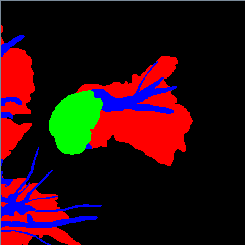
\includegraphics{img/fig_weights_normal.png}
	\end {subfigure}\hspace{2.5cm}
	\begin {subfigure}[b]{0.3\linewidth}
		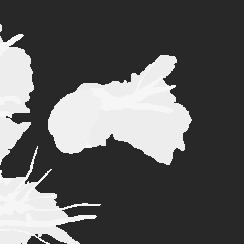
\includegraphics{img/fig_weights_weightmap.png}
	\end {subfigure}
	\end{center}

		\caption[The Cross-Entropy Loss weight map.]{\textbf{Left:} A ground truth label for an image with four classes, three of which are foreground classes. \textbf{Right:} The calculated weight map to use with the Weighted Cross-Entropy loss, created with inverse average weights and no distance modifier term. There are more background than foreground pixels, so the background is assigned a lower (darker) weight value, while the cell parts in the foreground are weighted heavier.}
		\label{fig:weight_map}

\end {figure}

\noindent The calculation of the $\delta$ value for Backpropagation is defined as follows:\footnote{The usual index $j$ for $\delta$ was omitted here and in the derivative of the Softmax because there is only one neuron in the loss layer anyway. Here, $j$ instead refers to the $j$th element of the vector $a$.}


\begin {align}
	\delta &= \frac{\partial \text{CE}}{\partial a_j} \\
		&= \frac{\partial}{\partial a_j} \left ( w \left ( - \sum \limits_{j=1}^{C} t_j \ln(y_j) \right ) \right ) \\ \intertext{where $w$ refers to the weight constant, $t_j$ is the ground truth probability and $y_j$ is the Softmax probability for the current pixel. Then}
		\delta &= w \left ( - \sum \limits_{j=1}^{C} t_j \frac{\partial \ln(y_j)}{\partial a_j} \right ) \\
		&= w \left (- \sum \limits_{j=1}^{C} t_j \frac{1}{y_j} \frac{\partial y_j}{\partial a_j} \right ) \\
		&= w \left ( - \frac{t_i}{y_i} \frac{\partial y_i}{\partial a_j} - \sum \limits_{j \neq i}^{C} \frac{t_j}{y_j} \frac{\partial y_j}{\partial a_j} \right ) \\ \intertext{using the derivative of the Softmax from Equation \textbf{\ref{eq:softmax_deriv}}, it follows that}
		\delta &= w \left ( - \frac{t_i}{y_i} y_i (1 - y_i) - \sum \limits_{j \neq i}^{C} \frac{t_j}{y_j} (- y_j y_i) \right ) \\
		&= w \left ( - t_i + t_i y_i - \sum \limits_{j \neq i}^{C} - t_j y_i \right ) \\
		&= w \left ( - t_i - \sum \limits_{j=1}^{C} - t_j y_i  \right ) \\
		&= w \left ( - t_i + y_i \sum \limits_{j=1}^{C} t_j \right ) \\ \intertext{Because $t_j = 0$ for all $C_j$ except the ground truth class, this can be simplified to} 
		\delta &= w \left (- t_i + y_i \right )
\end {align}

\noindent which is almost the same as the derivative of the normal Cross-Entropy loss.


		\subsection{F-Measure}
\label{subsec:fmeasure}

An alternative to solving the problem of unbalanced classes in the training data is using the \textit{F-Measure}, also called \textit{DICE similarity}, as a loss function instead. The F-Measure is a statistical similarity function which has been shown to perform well when using SGD-trained CNNs on unbalanced data for binary segmentations. \cite{fmeasure3, fmeasure5} It is based on the quantities of \textit{Precision} and \textit{Recall} over the training sample in comparison to its ground truth. The precision is defined as

\[ \text{PR} = \frac{\text{TP}}{\text{TP} + \text{FP}} \]

\noindent whereas the recall is defined as

\[ \text{RC} = \frac{\text{TP}}{\text{TP} + \text{FN}} \,, \]

\noindent where TP is the number of true positives, FP is the number of false positives, and FN is the number of false negatives. Traditionally, these values are defined as set theory operations, but to make the F-Measure differentiable, they are redefined as follows:

\begin {align}
\text{TP} &= \sum \limits_{i=1}^{n} y_i t_i \\
\text{FP} &= \sum  \limits_{i=1}^{n} y_i (1 - t_i) \\
\text{FN} &= \sum \limits_{i=1}^{n} (1 - y_i) t_i \,.
\end {align}

\noindent Here, $y_i$ and $t_i$ are the Softmax probability of the foreground class and the corresponding ground truth probability of a pixel $i$ in an image with $n$ pixels. The $F_1$ score for an image is then defined as

\begin {align}
 	F_1 &= 2 \left ( \frac{\text{PR} \cdot \text{RC}}{\text{PR} + \text{RC}} \right ) \\
		&= 2 \left ( \frac{\sum_{i=1}^{n} y_i t_i }{ \sum_{i=1}^{n} (y_i + t_i) } \right ) \,,
\end {align}

\noindent and the derivative to use during Backpropagation is

\begin {align}
	\delta &= \frac{\partial F_1}{\partial y_j}\\
	&= 2 \left ( \frac{t_j \sum_{i=1}^{n} \left ( y_i + t_i \right ) - \sum_{i=1}^{n} \left ( y_i t_i \right )  }{\left [ \sum_{i=1}^{n} \left ( y_i + t_i \right ) \right ]^2 } \right ) \,.
\end {align}

\noindent For multi-class problems, the approach is changed slightly: The $F_1$ score is calculated for each class $C_j$ in a binary fashion, using the $C_j$ as the ``foreground'' and all other classes $C_i, i \neq j$ as ``background''. This way, the definitions for TP, FP and FN can be used for more than two classes. The average of these multiple F-Measures is then used as the loss function.\footnote{It should be noted that the $F_1$ score \textbf{increases} the better the classification becomes.}

During the backward pass, the gradients are also calculated per class in a similiar way.


	\section {U-Net}
\label{sec:unet}
The U-Net \cite{unet} is a CNN architecture which aims to produce segmentation maps for images of cells. It was implemented using Caffe \cite{caffe}, a CNN library that allows CNN layers - such as the ones described in the previous section - to be put together to form a network.\\

The U-Net first performs a series of standard computations, alternating $3 \times 3$ convolutions followed by ReLU activations and $2 \times 2$ Maximum Pooling downsampling operations with stride $2$ while steadily increasing the number of filters after each pooling operation from 64 up to 1024. It differs from normal CNNs in that it then begins alternating stride $2 \times 2$ upsampling operations with $3 \times 3$ convolutions and thus enlarges the feature maps again while reducing the number of filters in a way that parallels the downsampling by Maximum Pooling. This results in a nearly symmetric architecture which gives the network its name. The upsampling operations are often called \textit{deconvolution layers}, and the way they work for upsampling by a factor of two in both dimensions can be thought of as padding the image with a zero-border with a width of one, while also inserting additional zero values inbetween the original values and then convoluting the resulting image normally with a stride of 1, using a $2 \times 2$ kernel. This approximately reverses the Maximum Pooling operation (see Figure \textbf{\ref{fig:upconvolution}}). \cite[p. 14]{transposed_conv}\cite{up_conv}

\begin {figure}[!hbt]
	\begin{center}
		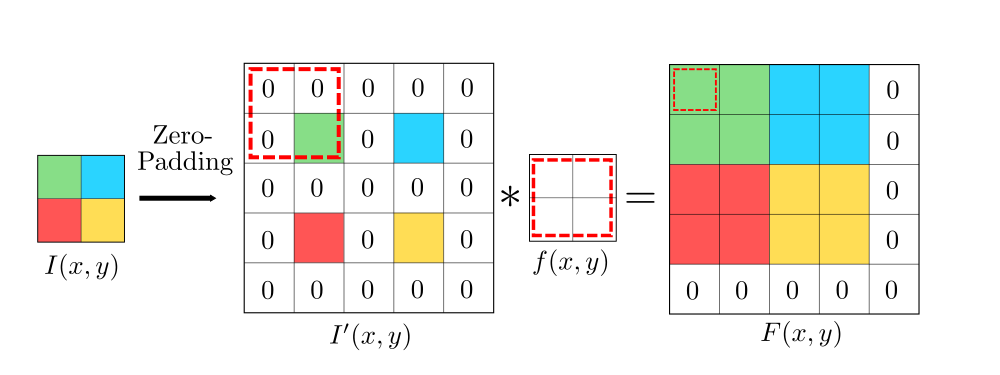
\includegraphics[scale=0.50]{img/fig_upconvolution}
	\end{center}
	\caption[Matrix upconvolution.]{The deconvolution or upsampling operation. This example shows upsampling by a factor of two of an input $I$, which is first padded with zero values to create $I'$, and then is convoluted with the $2 \times 2$ filter $f$. In this example, the ``center'' of the convolution is assumed to be the top left value. The dashed, red squares show the neighborhood of the first convolution step on $I'$ and the corresponding output in $F$. The additional zero values in $F$ can then be discarded, resulting in a approximate inversion of the Maximum Pooling operation. \footnotemark}
	\label{fig:upconvolution}
\end {figure}

 \footnotetext{While zero-padding works well to explain the idea behind the operation, the concept of \textit{transposed convolutions}, as described in \cite[p. 18]{transposed_conv} and \cite{up_conv} is used in frameworks like Caffe because it is more computationally efficient.}

The network is also a fully-convolutional network, so it does not have a final fully-connected layer. Instead, in order to classify each pixel, a $1 \times 1$ convolution with a number of filters that corresponds to the number of classes in the final segmentation map is used.

Additionally, the network allows feature concatenation by using shortcut connections (called ``skip-layer connections'' in \cite{bishop_pattern}), taking the non-padded part of the feature maps from the corresponding sampling level after each upsampling operation and concatenating them with the upsampled maps. This is done to boost the precision of the segmentation output - downsampling reduces locality information, which is nonetheless needed when creating a high-definition segmentation map, so this is a way to reduce the complexity of the network while still achieving precise results (see Figure \textbf{\ref{fig:unet_arch}} for a graphical representation of the U-Net architecture).\\

\begin {figure}[!htb]
	\scalebox{0.75}{\input{img/unet_arch.pdf_tex}}
	\caption[The U-Net architecture.]{The U-Net architecture. The white numbers indicate the number of filters per convolution, while the orange numbers show the number of feature maps that are taken from earlier layers for concatenation \textbf{before} downsampling is performed. In this example, the input is a grayscale image and therefore has one channel only. $C$ is the number of output classes to segment the image into, i.e. 3 or 4 depending on which dataset is used.}
	\label{fig:unet_arch}
\end {figure}
